\documentclass[twoside]{book}

% Packages required by doxygen
\usepackage{fixltx2e}
\usepackage{calc}
\usepackage{doxygen}
\usepackage[export]{adjustbox} % also loads graphicx
\usepackage{graphicx}
\usepackage[utf8]{inputenc}
\usepackage{makeidx}
\usepackage{multicol}
\usepackage{multirow}
\PassOptionsToPackage{warn}{textcomp}
\usepackage{textcomp}
\usepackage[nointegrals]{wasysym}
\usepackage[table]{xcolor}

% Font selection
\usepackage[T1]{fontenc}
\usepackage[scaled=.90]{helvet}
\usepackage{courier}
\usepackage{amssymb}
\usepackage{sectsty}
\renewcommand{\familydefault}{\sfdefault}
\allsectionsfont{%
  \fontseries{bc}\selectfont%
  \color{darkgray}%
}
\renewcommand{\DoxyLabelFont}{%
  \fontseries{bc}\selectfont%
  \color{darkgray}%
}
\newcommand{\+}{\discretionary{\mbox{\scriptsize$\hookleftarrow$}}{}{}}

% Page & text layout
\usepackage{geometry}
\geometry{%
  a4paper,%
  top=2.5cm,%
  bottom=2.5cm,%
  left=2.5cm,%
  right=2.5cm%
}
\tolerance=750
\hfuzz=15pt
\hbadness=750
\setlength{\emergencystretch}{15pt}
\setlength{\parindent}{0cm}
\setlength{\parskip}{3ex plus 2ex minus 2ex}
\makeatletter
\renewcommand{\paragraph}{%
  \@startsection{paragraph}{4}{0ex}{-1.0ex}{1.0ex}{%
    \normalfont\normalsize\bfseries\SS@parafont%
  }%
}
\renewcommand{\subparagraph}{%
  \@startsection{subparagraph}{5}{0ex}{-1.0ex}{1.0ex}{%
    \normalfont\normalsize\bfseries\SS@subparafont%
  }%
}
\makeatother

% Headers & footers
\usepackage{fancyhdr}
\pagestyle{fancyplain}
\fancyhead[LE]{\fancyplain{}{\bfseries\thepage}}
\fancyhead[CE]{\fancyplain{}{}}
\fancyhead[RE]{\fancyplain{}{\bfseries\leftmark}}
\fancyhead[LO]{\fancyplain{}{\bfseries\rightmark}}
\fancyhead[CO]{\fancyplain{}{}}
\fancyhead[RO]{\fancyplain{}{\bfseries\thepage}}
\fancyfoot[LE]{\fancyplain{}{}}
\fancyfoot[CE]{\fancyplain{}{}}
\fancyfoot[RE]{\fancyplain{}{\bfseries\scriptsize Generated by Doxygen }}
\fancyfoot[LO]{\fancyplain{}{\bfseries\scriptsize Generated by Doxygen }}
\fancyfoot[CO]{\fancyplain{}{}}
\fancyfoot[RO]{\fancyplain{}{}}
\renewcommand{\footrulewidth}{0.4pt}
\renewcommand{\chaptermark}[1]{%
  \markboth{#1}{}%
}
\renewcommand{\sectionmark}[1]{%
  \markright{\thesection\ #1}%
}

% Indices & bibliography
\usepackage{natbib}
\usepackage[titles]{tocloft}
\setcounter{tocdepth}{3}
\setcounter{secnumdepth}{5}
\makeindex

% Hyperlinks (required, but should be loaded last)
\usepackage{ifpdf}
\ifpdf
  \usepackage[pdftex,pagebackref=true]{hyperref}
\else
  \usepackage[ps2pdf,pagebackref=true]{hyperref}
\fi
\hypersetup{%
  colorlinks=true,%
  linkcolor=blue,%
  citecolor=blue,%
  unicode%
}

% Custom commands
\newcommand{\clearemptydoublepage}{%
  \newpage{\pagestyle{empty}\cleardoublepage}%
}

\usepackage{caption}
\captionsetup{labelsep=space,justification=centering,font={bf},singlelinecheck=off,skip=4pt,position=top}

%===== C O N T E N T S =====

\begin{document}

% Titlepage & ToC
\hypersetup{pageanchor=false,
             bookmarksnumbered=true,
             pdfencoding=unicode
            }
\pagenumbering{alph}
\begin{titlepage}
\vspace*{7cm}
\begin{center}%
{\Large Git\+Repo\+Cmdlet \\[1ex]\large 0.\+1b }\\
\vspace*{1cm}
{\large Generated by Doxygen 1.8.14}\\
\end{center}
\end{titlepage}
\clearemptydoublepage
\pagenumbering{roman}
\tableofcontents
\clearemptydoublepage
\pagenumbering{arabic}
\hypersetup{pageanchor=true}

%--- Begin generated contents ---
\chapter{Namespace Index}
\section{Packages}
Here are the packages with brief descriptions (if available)\+:\begin{DoxyCompactList}
\item\contentsline{section}{\mbox{\hyperlink{namespace_get_repo_cmdlet}{Get\+Repo\+Cmdlet}} }{\pageref{namespace_get_repo_cmdlet}}{}
\end{DoxyCompactList}

\chapter{Hierarchical Index}
\section{Class Hierarchy}
This inheritance list is sorted roughly, but not completely, alphabetically\+:\begin{DoxyCompactList}
\item \contentsline{section}{Get\+Repo\+Cmdlet.\+Cmd\+Container}{\pageref{class_get_repo_cmdlet_1_1_cmd_container}}{}
\item \contentsline{section}{Get\+Repo\+Cmdlet.\+Const\+Mgr}{\pageref{class_get_repo_cmdlet_1_1_const_mgr}}{}
\item \contentsline{section}{Get\+Repo\+Cmdlet.\+Enumerations}{\pageref{class_get_repo_cmdlet_1_1_enumerations}}{}
\item Exception\begin{DoxyCompactList}
\item \contentsline{section}{Get\+Repo\+Cmdlet.\+Invalid\+Git\+Repo\+Exception}{\pageref{class_get_repo_cmdlet_1_1_invalid_git_repo_exception}}{}
\end{DoxyCompactList}
\item \contentsline{section}{Get\+Repo\+Cmdlet.\+Processor}{\pageref{class_get_repo_cmdlet_1_1_processor}}{}
\item P\+S\+Cmdlet\begin{DoxyCompactList}
\item \contentsline{section}{Get\+Repo\+Cmdlet.\+Get\+Repo\+Cmdlet}{\pageref{class_get_repo_cmdlet_1_1_get_repo_cmdlet}}{}
\end{DoxyCompactList}
\end{DoxyCompactList}

\chapter{Class Index}
\section{Class List}
Here are the classes, structs, unions and interfaces with brief descriptions\+:\begin{DoxyCompactList}
\item\contentsline{section}{\mbox{\hyperlink{class_g_f_s_c_1_1_services_1_1_end_of_term_1_1_business_1_1_asset_information}{G\+F\+S\+C.\+Services.\+End\+Of\+Term.\+Business.\+Asset\+Information}} }{\pageref{class_g_f_s_c_1_1_services_1_1_end_of_term_1_1_business_1_1_asset_information}}{}
\item\contentsline{section}{\mbox{\hyperlink{class_g_f_s_c_1_1_services_1_1_end_of_term_1_1_data_1_1_asset_information}{G\+F\+S\+C.\+Services.\+End\+Of\+Term.\+Data.\+Asset\+Information}} }{\pageref{class_g_f_s_c_1_1_services_1_1_end_of_term_1_1_data_1_1_asset_information}}{}
\item\contentsline{section}{\mbox{\hyperlink{class_get_repo_cmdlet_1_1_cmd_container}{Get\+Repo\+Cmdlet.\+Cmd\+Container}} \\*Container for information needed to complete cmdlet processing. }{\pageref{class_get_repo_cmdlet_1_1_cmd_container}}{}
\item\contentsline{section}{\mbox{\hyperlink{class_get_repo_cmdlet_1_1_const_mgr}{Get\+Repo\+Cmdlet.\+Const\+Mgr}} \\*Contains constant values to be referenced throughout the cmdlet. All fields within this class can be altered and recompiled to create dynamic messages. }{\pageref{class_get_repo_cmdlet_1_1_const_mgr}}{}
\item\contentsline{section}{\mbox{\hyperlink{class_g_f_s_c_1_1_services_1_1_end_of_term_1_1_business_1_1_contract_information}{G\+F\+S\+C.\+Services.\+End\+Of\+Term.\+Business.\+Contract\+Information}} }{\pageref{class_g_f_s_c_1_1_services_1_1_end_of_term_1_1_business_1_1_contract_information}}{}
\item\contentsline{section}{\mbox{\hyperlink{class_g_f_s_c_1_1_services_1_1_end_of_term_1_1_data_1_1_contract_information}{G\+F\+S\+C.\+Services.\+End\+Of\+Term.\+Data.\+Contract\+Information}} }{\pageref{class_g_f_s_c_1_1_services_1_1_end_of_term_1_1_data_1_1_contract_information}}{}
\item\contentsline{section}{\mbox{\hyperlink{class_g_f_s_c_1_1_services_1_1_end_of_term_1_1_data_1_1_customer_information}{G\+F\+S\+C.\+Services.\+End\+Of\+Term.\+Data.\+Customer\+Information}} }{\pageref{class_g_f_s_c_1_1_services_1_1_end_of_term_1_1_data_1_1_customer_information}}{}
\item\contentsline{section}{\mbox{\hyperlink{class_g_f_s_c_1_1_services_1_1_end_of_term_1_1_business_1_1_customer_information}{G\+F\+S\+C.\+Services.\+End\+Of\+Term.\+Business.\+Customer\+Information}} }{\pageref{class_g_f_s_c_1_1_services_1_1_end_of_term_1_1_business_1_1_customer_information}}{}
\item\contentsline{section}{\mbox{\hyperlink{class_g_f_s_c_1_1_services_1_1_end_of_term_1_1_business_1_1_dealer_information}{G\+F\+S\+C.\+Services.\+End\+Of\+Term.\+Business.\+Dealer\+Information}} }{\pageref{class_g_f_s_c_1_1_services_1_1_end_of_term_1_1_business_1_1_dealer_information}}{}
\item\contentsline{section}{\mbox{\hyperlink{class_g_f_s_c_1_1_services_1_1_end_of_term_1_1_data_1_1_dealer_information}{G\+F\+S\+C.\+Services.\+End\+Of\+Term.\+Data.\+Dealer\+Information}} }{\pageref{class_g_f_s_c_1_1_services_1_1_end_of_term_1_1_data_1_1_dealer_information}}{}
\item\contentsline{section}{\mbox{\hyperlink{class_g_f_s_c_1_1_services_1_1_end_of_term_1_1_end_of_term_service}{G\+F\+S\+C.\+Services.\+End\+Of\+Term.\+End\+Of\+Term\+Service}} }{\pageref{class_g_f_s_c_1_1_services_1_1_end_of_term_1_1_end_of_term_service}}{}
\item\contentsline{section}{\mbox{\hyperlink{class_get_repo_cmdlet_1_1_enumerations}{Get\+Repo\+Cmdlet.\+Enumerations}} \\*Contains enumerations to be used throughout the cmdlet. }{\pageref{class_get_repo_cmdlet_1_1_enumerations}}{}
\item\contentsline{section}{\mbox{\hyperlink{class_g_f_s_c_1_1_services_1_1_end_of_term_1_1_i_m_service_1_1_execute_integration_manager_call_completed_event_args}{G\+F\+S\+C.\+Services.\+End\+Of\+Term.\+I\+M\+Service.\+Execute\+Integration\+Manager\+Call\+Completed\+Event\+Args}} \\*}{\pageref{class_g_f_s_c_1_1_services_1_1_end_of_term_1_1_i_m_service_1_1_execute_integration_manager_call_completed_event_args}}{}
\item\contentsline{section}{\mbox{\hyperlink{class_g_f_s_c_1_1_services_1_1_end_of_term_1_1_i_m_service_1_1_execute_u_r_l_completed_event_args}{G\+F\+S\+C.\+Services.\+End\+Of\+Term.\+I\+M\+Service.\+Execute\+U\+R\+L\+Completed\+Event\+Args}} \\*}{\pageref{class_g_f_s_c_1_1_services_1_1_end_of_term_1_1_i_m_service_1_1_execute_u_r_l_completed_event_args}}{}
\item\contentsline{section}{\mbox{\hyperlink{class_g_f_s_c_1_1_services_1_1_test_application_1_1_form1}{G\+F\+S\+C.\+Services.\+Test\+Application.\+Form1}} }{\pageref{class_g_f_s_c_1_1_services_1_1_test_application_1_1_form1}}{}
\item\contentsline{section}{\mbox{\hyperlink{class_get_repo_cmdlet_1_1_get_repo_cmdlet}{Get\+Repo\+Cmdlet.\+Get\+Repo\+Cmdlet}} \\*Cmdlet definition class to create Get-\/\+Repo cmdlet. }{\pageref{class_get_repo_cmdlet_1_1_get_repo_cmdlet}}{}
\item\contentsline{section}{\mbox{\hyperlink{interface_g_f_s_c_1_1_services_1_1_end_of_term_1_1_i_end_of_term_service}{G\+F\+S\+C.\+Services.\+End\+Of\+Term.\+I\+End\+Of\+Term\+Service}} }{\pageref{interface_g_f_s_c_1_1_services_1_1_end_of_term_1_1_i_end_of_term_service}}{}
\item\contentsline{section}{\mbox{\hyperlink{class_g_f_s_c_1_1_services_1_1_end_of_term_1_1_i_m_service_1_1_i_m_service}{G\+F\+S\+C.\+Services.\+End\+Of\+Term.\+I\+M\+Service.\+I\+M\+Service}} \\*}{\pageref{class_g_f_s_c_1_1_services_1_1_end_of_term_1_1_i_m_service_1_1_i_m_service}}{}
\item\contentsline{section}{\mbox{\hyperlink{class_get_repo_cmdlet_1_1_invalid_git_repo_exception}{Get\+Repo\+Cmdlet.\+Invalid\+Git\+Repo\+Exception}} \\*Custom application exception to handle invalid entries in the Git\+Repo parameter. }{\pageref{class_get_repo_cmdlet_1_1_invalid_git_repo_exception}}{}
\item\contentsline{section}{\mbox{\hyperlink{interface_g_f_s_c_1_1_services_1_1_end_of_term_1_1_i_quotes}{G\+F\+S\+C.\+Services.\+End\+Of\+Term.\+I\+Quotes}} \\*Quote Interface }{\pageref{interface_g_f_s_c_1_1_services_1_1_end_of_term_1_1_i_quotes}}{}
\item\contentsline{section}{\mbox{\hyperlink{class_g_f_s_c_1_1_services_1_1_end_of_term_1_1_misc_fee}{G\+F\+S\+C.\+Services.\+End\+Of\+Term.\+Misc\+Fee}} \\*Miscellaneous fee associated with a quote }{\pageref{class_g_f_s_c_1_1_services_1_1_end_of_term_1_1_misc_fee}}{}
\item\contentsline{section}{\mbox{\hyperlink{class_g_f_s_c_1_1_services_1_1_end_of_term_1_1_business_1_1_misc_information}{G\+F\+S\+C.\+Services.\+End\+Of\+Term.\+Business.\+Misc\+Information}} }{\pageref{class_g_f_s_c_1_1_services_1_1_end_of_term_1_1_business_1_1_misc_information}}{}
\item\contentsline{section}{\mbox{\hyperlink{class_g_f_s_c_1_1_services_1_1_end_of_term_1_1_data_1_1_misc_information}{G\+F\+S\+C.\+Services.\+End\+Of\+Term.\+Data.\+Misc\+Information}} }{\pageref{class_g_f_s_c_1_1_services_1_1_end_of_term_1_1_data_1_1_misc_information}}{}
\item\contentsline{section}{\mbox{\hyperlink{class_get_repo_cmdlet_1_1_processor}{Get\+Repo\+Cmdlet.\+Processor}} \\*Internal static class that holds logic for execution of the cmdlet. }{\pageref{class_get_repo_cmdlet_1_1_processor}}{}
\item\contentsline{section}{\mbox{\hyperlink{class_g_f_s_c_1_1_services_1_1_test_application_1_1_program}{G\+F\+S\+C.\+Services.\+Test\+Application.\+Program}} }{\pageref{class_g_f_s_c_1_1_services_1_1_test_application_1_1_program}}{}
\item\contentsline{section}{\mbox{\hyperlink{class_g_f_s_c_1_1_services_1_1_end_of_term_1_1_quote_details}{G\+F\+S\+C.\+Services.\+End\+Of\+Term.\+Quote\+Details}} \\*All information pertaining to a quote }{\pageref{class_g_f_s_c_1_1_services_1_1_end_of_term_1_1_quote_details}}{}
\item\contentsline{section}{\mbox{\hyperlink{class_g_f_s_c_1_1_services_1_1_end_of_term_1_1_quote_info}{G\+F\+S\+C.\+Services.\+End\+Of\+Term.\+Quote\+Info}} \\*Type of quote }{\pageref{class_g_f_s_c_1_1_services_1_1_end_of_term_1_1_quote_info}}{}
\item\contentsline{section}{\mbox{\hyperlink{class_g_f_s_c_1_1_services_1_1_end_of_term_1_1_data_1_1_quote_information}{G\+F\+S\+C.\+Services.\+End\+Of\+Term.\+Data.\+Quote\+Information}} }{\pageref{class_g_f_s_c_1_1_services_1_1_end_of_term_1_1_data_1_1_quote_information}}{}
\item\contentsline{section}{\mbox{\hyperlink{class_g_f_s_c_1_1_services_1_1_end_of_term_1_1_business_1_1_quote_information}{G\+F\+S\+C.\+Services.\+End\+Of\+Term.\+Business.\+Quote\+Information}} }{\pageref{class_g_f_s_c_1_1_services_1_1_end_of_term_1_1_business_1_1_quote_information}}{}
\item\contentsline{section}{\mbox{\hyperlink{class_g_f_s_c_1_1_services_1_1_end_of_term_1_1_quote_request}{G\+F\+S\+C.\+Services.\+End\+Of\+Term.\+Quote\+Request}} \\*\mbox{\hyperlink{namespace_g_f_s_c_1_1_services_1_1_end_of_term_1_1_data}{Data}} necessary for creating a quote }{\pageref{class_g_f_s_c_1_1_services_1_1_end_of_term_1_1_quote_request}}{}
\item\contentsline{section}{\mbox{\hyperlink{class_g_f_s_c_1_1_services_1_1_end_of_term_1_1_quote_return}{G\+F\+S\+C.\+Services.\+End\+Of\+Term.\+Quote\+Return}} \\*Quote ID or Error message when a quote is calculated }{\pageref{class_g_f_s_c_1_1_services_1_1_end_of_term_1_1_quote_return}}{}
\item\contentsline{section}{\mbox{\hyperlink{class_g_f_s_c_1_1_services_1_1_end_of_term_1_1_quotes}{G\+F\+S\+C.\+Services.\+End\+Of\+Term.\+Quotes}} \\*Methods for quotes }{\pageref{class_g_f_s_c_1_1_services_1_1_end_of_term_1_1_quotes}}{}
\item\contentsline{section}{\mbox{\hyperlink{class_g_f_s_c_1_1_services_1_1_end_of_term_1_1_quote_view}{G\+F\+S\+C.\+Services.\+End\+Of\+Term.\+Quote\+View}} \\*\mbox{\hyperlink{namespace_g_f_s_c_1_1_services_1_1_end_of_term_1_1_data}{Data}} required to view a quote }{\pageref{class_g_f_s_c_1_1_services_1_1_end_of_term_1_1_quote_view}}{}
\item\contentsline{section}{\mbox{\hyperlink{class_g_f_s_c_1_1_services_1_1_test_application_1_1_properties_1_1_resources}{G\+F\+S\+C.\+Services.\+Test\+Application.\+Properties.\+Resources}} \\*A strongly-\/typed resource class, for looking up localized strings, etc. }{\pageref{class_g_f_s_c_1_1_services_1_1_test_application_1_1_properties_1_1_resources}}{}
\item\contentsline{section}{\mbox{\hyperlink{class_g_f_s_c_1_1_services_1_1_end_of_term_1_1_properties_1_1_settings}{G\+F\+S\+C.\+Services.\+End\+Of\+Term.\+Properties.\+Settings}} }{\pageref{class_g_f_s_c_1_1_services_1_1_end_of_term_1_1_properties_1_1_settings}}{}
\item\contentsline{section}{\mbox{\hyperlink{class_g_f_s_c_1_1_services_1_1_test_application_1_1_properties_1_1_settings}{G\+F\+S\+C.\+Services.\+Test\+Application.\+Properties.\+Settings}} }{\pageref{class_g_f_s_c_1_1_services_1_1_test_application_1_1_properties_1_1_settings}}{}
\item\contentsline{section}{\mbox{\hyperlink{class_g_f_s_c_1_1_services_1_1_end_of_term_1_1_data_1_1_unpaid_open_item_information}{G\+F\+S\+C.\+Services.\+End\+Of\+Term.\+Data.\+Unpaid\+Open\+Item\+Information}} }{\pageref{class_g_f_s_c_1_1_services_1_1_end_of_term_1_1_data_1_1_unpaid_open_item_information}}{}
\end{DoxyCompactList}

\chapter{File Index}
\section{File List}
Here is a list of all files with brief descriptions\+:\begin{DoxyCompactList}
\item\contentsline{section}{Get\+Repo\+Cmdlet/\mbox{\hyperlink{_get_repo_cmdlet_8_const_mgr_8cs}{Get\+Repo\+Cmdlet.\+Const\+Mgr.\+cs}} }{\pageref{_get_repo_cmdlet_8_const_mgr_8cs}}{}
\item\contentsline{section}{Get\+Repo\+Cmdlet/\mbox{\hyperlink{_get_repo_cmdlet_8cs}{Get\+Repo\+Cmdlet.\+cs}} }{\pageref{_get_repo_cmdlet_8cs}}{}
\item\contentsline{section}{Get\+Repo\+Cmdlet/\mbox{\hyperlink{_get_repo_cmdlet_8_objects_8cs}{Get\+Repo\+Cmdlet.\+Objects.\+cs}} }{\pageref{_get_repo_cmdlet_8_objects_8cs}}{}
\item\contentsline{section}{Get\+Repo\+Cmdlet/\mbox{\hyperlink{_get_repo_cmdlet_8_processor_8cs}{Get\+Repo\+Cmdlet.\+Processor.\+cs}} }{\pageref{_get_repo_cmdlet_8_processor_8cs}}{}
\item\contentsline{section}{Get\+Repo\+Cmdlet/bin/\+Debug/\+G\+F\+S\+C.\+Services.\+End\+Of\+Term/\+G\+F\+S\+C.\+Services.\+End\+Of\+Term/\mbox{\hyperlink{_end_of_term_service_8svc_8cs}{End\+Of\+Term\+Service.\+svc.\+cs}} }{\pageref{_end_of_term_service_8svc_8cs}}{}
\item\contentsline{section}{Get\+Repo\+Cmdlet/bin/\+Debug/\+G\+F\+S\+C.\+Services.\+End\+Of\+Term/\+G\+F\+S\+C.\+Services.\+End\+Of\+Term/\mbox{\hyperlink{_i_end_of_term_service_8cs}{I\+End\+Of\+Term\+Service.\+cs}} }{\pageref{_i_end_of_term_service_8cs}}{}
\item\contentsline{section}{Get\+Repo\+Cmdlet/bin/\+Debug/\+G\+F\+S\+C.\+Services.\+End\+Of\+Term/\+G\+F\+S\+C.\+Services.\+End\+Of\+Term/\mbox{\hyperlink{_i_quotes_8cs}{I\+Quotes.\+cs}} }{\pageref{_i_quotes_8cs}}{}
\item\contentsline{section}{Get\+Repo\+Cmdlet/bin/\+Debug/\+G\+F\+S\+C.\+Services.\+End\+Of\+Term/\+G\+F\+S\+C.\+Services.\+End\+Of\+Term/\mbox{\hyperlink{_quotes_8svc_8cs}{Quotes.\+svc.\+cs}} }{\pageref{_quotes_8svc_8cs}}{}
\item\contentsline{section}{Get\+Repo\+Cmdlet/bin/\+Debug/\+G\+F\+S\+C.\+Services.\+End\+Of\+Term/\+G\+F\+S\+C.\+Services.\+End\+Of\+Term/\+Business/\mbox{\hyperlink{_business_2_asset_information_8cs}{Asset\+Information.\+cs}} }{\pageref{_business_2_asset_information_8cs}}{}
\item\contentsline{section}{Get\+Repo\+Cmdlet/bin/\+Debug/\+G\+F\+S\+C.\+Services.\+End\+Of\+Term/\+G\+F\+S\+C.\+Services.\+End\+Of\+Term/\+Business/\mbox{\hyperlink{_business_2_contract_information_8cs}{Contract\+Information.\+cs}} }{\pageref{_business_2_contract_information_8cs}}{}
\item\contentsline{section}{Get\+Repo\+Cmdlet/bin/\+Debug/\+G\+F\+S\+C.\+Services.\+End\+Of\+Term/\+G\+F\+S\+C.\+Services.\+End\+Of\+Term/\+Business/\mbox{\hyperlink{_business_2_customer_information_8cs}{Customer\+Information.\+cs}} }{\pageref{_business_2_customer_information_8cs}}{}
\item\contentsline{section}{Get\+Repo\+Cmdlet/bin/\+Debug/\+G\+F\+S\+C.\+Services.\+End\+Of\+Term/\+G\+F\+S\+C.\+Services.\+End\+Of\+Term/\+Business/\mbox{\hyperlink{_business_2_dealer_information_8cs}{Dealer\+Information.\+cs}} }{\pageref{_business_2_dealer_information_8cs}}{}
\item\contentsline{section}{Get\+Repo\+Cmdlet/bin/\+Debug/\+G\+F\+S\+C.\+Services.\+End\+Of\+Term/\+G\+F\+S\+C.\+Services.\+End\+Of\+Term/\+Business/\mbox{\hyperlink{_business_2_misc_information_8cs}{Misc\+Information.\+cs}} }{\pageref{_business_2_misc_information_8cs}}{}
\item\contentsline{section}{Get\+Repo\+Cmdlet/bin/\+Debug/\+G\+F\+S\+C.\+Services.\+End\+Of\+Term/\+G\+F\+S\+C.\+Services.\+End\+Of\+Term/\+Business/\mbox{\hyperlink{_business_2_quote_information_8cs}{Quote\+Information.\+cs}} }{\pageref{_business_2_quote_information_8cs}}{}
\item\contentsline{section}{Get\+Repo\+Cmdlet/bin/\+Debug/\+G\+F\+S\+C.\+Services.\+End\+Of\+Term/\+G\+F\+S\+C.\+Services.\+End\+Of\+Term/\+Data/\mbox{\hyperlink{_data_2_asset_information_8cs}{Asset\+Information.\+cs}} }{\pageref{_data_2_asset_information_8cs}}{}
\item\contentsline{section}{Get\+Repo\+Cmdlet/bin/\+Debug/\+G\+F\+S\+C.\+Services.\+End\+Of\+Term/\+G\+F\+S\+C.\+Services.\+End\+Of\+Term/\+Data/\mbox{\hyperlink{_data_2_contract_information_8cs}{Contract\+Information.\+cs}} }{\pageref{_data_2_contract_information_8cs}}{}
\item\contentsline{section}{Get\+Repo\+Cmdlet/bin/\+Debug/\+G\+F\+S\+C.\+Services.\+End\+Of\+Term/\+G\+F\+S\+C.\+Services.\+End\+Of\+Term/\+Data/\mbox{\hyperlink{_data_2_customer_information_8cs}{Customer\+Information.\+cs}} }{\pageref{_data_2_customer_information_8cs}}{}
\item\contentsline{section}{Get\+Repo\+Cmdlet/bin/\+Debug/\+G\+F\+S\+C.\+Services.\+End\+Of\+Term/\+G\+F\+S\+C.\+Services.\+End\+Of\+Term/\+Data/\mbox{\hyperlink{_data_2_dealer_information_8cs}{Dealer\+Information.\+cs}} }{\pageref{_data_2_dealer_information_8cs}}{}
\item\contentsline{section}{Get\+Repo\+Cmdlet/bin/\+Debug/\+G\+F\+S\+C.\+Services.\+End\+Of\+Term/\+G\+F\+S\+C.\+Services.\+End\+Of\+Term/\+Data/\mbox{\hyperlink{_data_2_misc_information_8cs}{Misc\+Information.\+cs}} }{\pageref{_data_2_misc_information_8cs}}{}
\item\contentsline{section}{Get\+Repo\+Cmdlet/bin/\+Debug/\+G\+F\+S\+C.\+Services.\+End\+Of\+Term/\+G\+F\+S\+C.\+Services.\+End\+Of\+Term/\+Data/\mbox{\hyperlink{_data_2_quote_information_8cs}{Quote\+Information.\+cs}} }{\pageref{_data_2_quote_information_8cs}}{}
\item\contentsline{section}{Get\+Repo\+Cmdlet/bin/\+Debug/\+G\+F\+S\+C.\+Services.\+End\+Of\+Term/\+G\+F\+S\+C.\+Services.\+End\+Of\+Term/\+Data/\mbox{\hyperlink{_unpaid_open_item_information_8cs}{Unpaid\+Open\+Item\+Information.\+cs}} }{\pageref{_unpaid_open_item_information_8cs}}{}
\item\contentsline{section}{Get\+Repo\+Cmdlet/bin/\+Debug/\+G\+F\+S\+C.\+Services.\+End\+Of\+Term/\+G\+F\+S\+C.\+Services.\+End\+Of\+Term/\+Properties/\mbox{\hyperlink{bin_2_debug_2_g_f_s_c_8_services_8_end_of_term_2_g_f_s_c_8_services_8_end_of_term_2_properties_2_assembly_info_8cs}{Assembly\+Info.\+cs}} }{\pageref{bin_2_debug_2_g_f_s_c_8_services_8_end_of_term_2_g_f_s_c_8_services_8_end_of_term_2_properties_2_assembly_info_8cs}}{}
\item\contentsline{section}{Get\+Repo\+Cmdlet/bin/\+Debug/\+G\+F\+S\+C.\+Services.\+End\+Of\+Term/\+G\+F\+S\+C.\+Services.\+End\+Of\+Term/\+Properties/\mbox{\hyperlink{_g_f_s_c_8_services_8_end_of_term_2_properties_2_settings_8_designer_8cs}{Settings.\+Designer.\+cs}} }{\pageref{_g_f_s_c_8_services_8_end_of_term_2_properties_2_settings_8_designer_8cs}}{}
\item\contentsline{section}{Get\+Repo\+Cmdlet/bin/\+Debug/\+G\+F\+S\+C.\+Services.\+End\+Of\+Term/\+G\+F\+S\+C.\+Services.\+End\+Of\+Term/\+Web References/\+I\+M\+Service/\mbox{\hyperlink{_reference_8cs}{Reference.\+cs}} }{\pageref{_reference_8cs}}{}
\item\contentsline{section}{Get\+Repo\+Cmdlet/bin/\+Debug/\+G\+F\+S\+C.\+Services.\+End\+Of\+Term/\+G\+F\+S\+C.\+Services.\+Test\+Application/\mbox{\hyperlink{_form1_8cs}{Form1.\+cs}} }{\pageref{_form1_8cs}}{}
\item\contentsline{section}{Get\+Repo\+Cmdlet/bin/\+Debug/\+G\+F\+S\+C.\+Services.\+End\+Of\+Term/\+G\+F\+S\+C.\+Services.\+Test\+Application/\mbox{\hyperlink{_form1_8_designer_8cs}{Form1.\+Designer.\+cs}} }{\pageref{_form1_8_designer_8cs}}{}
\item\contentsline{section}{Get\+Repo\+Cmdlet/bin/\+Debug/\+G\+F\+S\+C.\+Services.\+End\+Of\+Term/\+G\+F\+S\+C.\+Services.\+Test\+Application/\mbox{\hyperlink{_program_8cs}{Program.\+cs}} }{\pageref{_program_8cs}}{}
\item\contentsline{section}{Get\+Repo\+Cmdlet/bin/\+Debug/\+G\+F\+S\+C.\+Services.\+End\+Of\+Term/\+G\+F\+S\+C.\+Services.\+Test\+Application/obj/\+Debug/\mbox{\hyperlink{bin_2_debug_2_g_f_s_c_8_services_8_end_of_term_2_g_f_s_c_8_services_8_test_application_2obj_2_de55f8097c839b93f948b34c88cde7635b}{Temporary\+Generated\+File\+\_\+036\+C0\+B5\+B-\/1481-\/4323-\/8\+D20-\/8\+F5\+A\+D\+C\+B23\+D92.\+cs}} }{\pageref{bin_2_debug_2_g_f_s_c_8_services_8_end_of_term_2_g_f_s_c_8_services_8_test_application_2obj_2_de55f8097c839b93f948b34c88cde7635b}}{}
\item\contentsline{section}{Get\+Repo\+Cmdlet/bin/\+Debug/\+G\+F\+S\+C.\+Services.\+End\+Of\+Term/\+G\+F\+S\+C.\+Services.\+Test\+Application/obj/\+Debug/\mbox{\hyperlink{bin_2_debug_2_g_f_s_c_8_services_8_end_of_term_2_g_f_s_c_8_services_8_test_application_2obj_2_def61a45030267eb98eecf5e3d82d134ae}{Temporary\+Generated\+File\+\_\+5937a670-\/0e60-\/4077-\/877b-\/f7221da3dda1.\+cs}} }{\pageref{bin_2_debug_2_g_f_s_c_8_services_8_end_of_term_2_g_f_s_c_8_services_8_test_application_2obj_2_def61a45030267eb98eecf5e3d82d134ae}}{}
\item\contentsline{section}{Get\+Repo\+Cmdlet/bin/\+Debug/\+G\+F\+S\+C.\+Services.\+End\+Of\+Term/\+G\+F\+S\+C.\+Services.\+Test\+Application/obj/\+Debug/\mbox{\hyperlink{bin_2_debug_2_g_f_s_c_8_services_8_end_of_term_2_g_f_s_c_8_services_8_test_application_2obj_2_def0e36264e6a95f86ac63762cb5927946}{Temporary\+Generated\+File\+\_\+\+E7\+A71\+F73-\/0\+F8\+D-\/4\+B9\+B-\/\+B56\+E-\/8\+E70\+B10\+B\+C5\+D3.\+cs}} }{\pageref{bin_2_debug_2_g_f_s_c_8_services_8_end_of_term_2_g_f_s_c_8_services_8_test_application_2obj_2_def0e36264e6a95f86ac63762cb5927946}}{}
\item\contentsline{section}{Get\+Repo\+Cmdlet/bin/\+Debug/\+G\+F\+S\+C.\+Services.\+End\+Of\+Term/\+G\+F\+S\+C.\+Services.\+Test\+Application/obj/\+Release/\mbox{\hyperlink{bin_2_debug_2_g_f_s_c_8_services_8_end_of_term_2_g_f_s_c_8_services_8_test_application_2obj_2_re303e4215acf599da6e8969bb4551eea7}{Temporary\+Generated\+File\+\_\+036\+C0\+B5\+B-\/1481-\/4323-\/8\+D20-\/8\+F5\+A\+D\+C\+B23\+D92.\+cs}} }{\pageref{bin_2_debug_2_g_f_s_c_8_services_8_end_of_term_2_g_f_s_c_8_services_8_test_application_2obj_2_re303e4215acf599da6e8969bb4551eea7}}{}
\item\contentsline{section}{Get\+Repo\+Cmdlet/bin/\+Debug/\+G\+F\+S\+C.\+Services.\+End\+Of\+Term/\+G\+F\+S\+C.\+Services.\+Test\+Application/obj/\+Release/\mbox{\hyperlink{bin_2_debug_2_g_f_s_c_8_services_8_end_of_term_2_g_f_s_c_8_services_8_test_application_2obj_2_re74c340a34fbd976ce4e8e746d4c34bbd}{Temporary\+Generated\+File\+\_\+5937a670-\/0e60-\/4077-\/877b-\/f7221da3dda1.\+cs}} }{\pageref{bin_2_debug_2_g_f_s_c_8_services_8_end_of_term_2_g_f_s_c_8_services_8_test_application_2obj_2_re74c340a34fbd976ce4e8e746d4c34bbd}}{}
\item\contentsline{section}{Get\+Repo\+Cmdlet/bin/\+Debug/\+G\+F\+S\+C.\+Services.\+End\+Of\+Term/\+G\+F\+S\+C.\+Services.\+Test\+Application/obj/\+Release/\mbox{\hyperlink{bin_2_debug_2_g_f_s_c_8_services_8_end_of_term_2_g_f_s_c_8_services_8_test_application_2obj_2_recfc08711b3188d6c6d16dab5300cb204}{Temporary\+Generated\+File\+\_\+\+E7\+A71\+F73-\/0\+F8\+D-\/4\+B9\+B-\/\+B56\+E-\/8\+E70\+B10\+B\+C5\+D3.\+cs}} }{\pageref{bin_2_debug_2_g_f_s_c_8_services_8_end_of_term_2_g_f_s_c_8_services_8_test_application_2obj_2_recfc08711b3188d6c6d16dab5300cb204}}{}
\item\contentsline{section}{Get\+Repo\+Cmdlet/bin/\+Debug/\+G\+F\+S\+C.\+Services.\+End\+Of\+Term/\+G\+F\+S\+C.\+Services.\+Test\+Application/\+Properties/\mbox{\hyperlink{bin_2_debug_2_g_f_s_c_8_services_8_end_of_term_2_g_f_s_c_8_services_8_test_application_2_properties_2_assembly_info_8cs}{Assembly\+Info.\+cs}} }{\pageref{bin_2_debug_2_g_f_s_c_8_services_8_end_of_term_2_g_f_s_c_8_services_8_test_application_2_properties_2_assembly_info_8cs}}{}
\item\contentsline{section}{Get\+Repo\+Cmdlet/bin/\+Debug/\+G\+F\+S\+C.\+Services.\+End\+Of\+Term/\+G\+F\+S\+C.\+Services.\+Test\+Application/\+Properties/\mbox{\hyperlink{_resources_8_designer_8cs}{Resources.\+Designer.\+cs}} }{\pageref{_resources_8_designer_8cs}}{}
\item\contentsline{section}{Get\+Repo\+Cmdlet/bin/\+Debug/\+G\+F\+S\+C.\+Services.\+End\+Of\+Term/\+G\+F\+S\+C.\+Services.\+Test\+Application/\+Properties/\mbox{\hyperlink{_g_f_s_c_8_services_8_test_application_2_properties_2_settings_8_designer_8cs}{Settings.\+Designer.\+cs}} }{\pageref{_g_f_s_c_8_services_8_test_application_2_properties_2_settings_8_designer_8cs}}{}
\item\contentsline{section}{Get\+Repo\+Cmdlet/obj/\+Debug/\mbox{\hyperlink{obj_2_debug_2_temporary_generated_file__036_c0_b5_b-1481-4323-8_d20-8_f5_a_d_c_b23_d92_8cs}{Temporary\+Generated\+File\+\_\+036\+C0\+B5\+B-\/1481-\/4323-\/8\+D20-\/8\+F5\+A\+D\+C\+B23\+D92.\+cs}} }{\pageref{obj_2_debug_2_temporary_generated_file__036_c0_b5_b-1481-4323-8_d20-8_f5_a_d_c_b23_d92_8cs}}{}
\item\contentsline{section}{Get\+Repo\+Cmdlet/obj/\+Debug/\mbox{\hyperlink{obj_2_debug_2_temporary_generated_file__5937a670-0e60-4077-877b-f7221da3dda1_8cs}{Temporary\+Generated\+File\+\_\+5937a670-\/0e60-\/4077-\/877b-\/f7221da3dda1.\+cs}} }{\pageref{obj_2_debug_2_temporary_generated_file__5937a670-0e60-4077-877b-f7221da3dda1_8cs}}{}
\item\contentsline{section}{Get\+Repo\+Cmdlet/obj/\+Debug/\mbox{\hyperlink{obj_2_debug_2_temporary_generated_file___e7_a71_f73-0_f8_d-4_b9_b-_b56_e-8_e70_b10_b_c5_d3_8cs}{Temporary\+Generated\+File\+\_\+\+E7\+A71\+F73-\/0\+F8\+D-\/4\+B9\+B-\/\+B56\+E-\/8\+E70\+B10\+B\+C5\+D3.\+cs}} }{\pageref{obj_2_debug_2_temporary_generated_file___e7_a71_f73-0_f8_d-4_b9_b-_b56_e-8_e70_b10_b_c5_d3_8cs}}{}
\item\contentsline{section}{Get\+Repo\+Cmdlet/\+Properties/\mbox{\hyperlink{_properties_2_assembly_info_8cs}{Assembly\+Info.\+cs}} }{\pageref{_properties_2_assembly_info_8cs}}{}
\end{DoxyCompactList}

\chapter{Namespace Documentation}
\hypertarget{namespace_get_repo_cmdlet}{}\section{Get\+Repo\+Cmdlet Namespace Reference}
\label{namespace_get_repo_cmdlet}\index{Get\+Repo\+Cmdlet@{Get\+Repo\+Cmdlet}}
\subsection*{Classes}
\begin{DoxyCompactItemize}
\item 
class \mbox{\hyperlink{class_get_repo_cmdlet_1_1_cmd_container}{Cmd\+Container}}
\begin{DoxyCompactList}\small\item\em Container for information needed to complete cmdlet processing. \end{DoxyCompactList}\item 
class \mbox{\hyperlink{class_get_repo_cmdlet_1_1_const_mgr}{Const\+Mgr}}
\begin{DoxyCompactList}\small\item\em Contains constant values to be referenced throughout the cmdlet. All fields within this class can be altered and recompiled to create dynamic messages. \end{DoxyCompactList}\item 
class \mbox{\hyperlink{class_get_repo_cmdlet_1_1_enumerations}{Enumerations}}
\begin{DoxyCompactList}\small\item\em Contains enumerations to be used throughout the cmdlet. \end{DoxyCompactList}\item 
class \mbox{\hyperlink{class_get_repo_cmdlet_1_1_get_repo_cmdlet}{Get\+Repo\+Cmdlet}}
\begin{DoxyCompactList}\small\item\em Cmdlet definition class to create Get-\/\+Repo cmdlet. \end{DoxyCompactList}\item 
class \mbox{\hyperlink{class_get_repo_cmdlet_1_1_invalid_git_repo_exception}{Invalid\+Git\+Repo\+Exception}}
\begin{DoxyCompactList}\small\item\em Custom application exception to handle invalid entries in the Git\+Repo parameter. \end{DoxyCompactList}\item 
class \mbox{\hyperlink{class_get_repo_cmdlet_1_1_processor}{Processor}}
\begin{DoxyCompactList}\small\item\em Internal static class that holds logic for execution of the cmdlet. \end{DoxyCompactList}\end{DoxyCompactItemize}

\chapter{Class Documentation}
\hypertarget{class_get_repo_cmdlet_1_1_cmd_container}{}\section{Get\+Repo\+Cmdlet.\+Cmd\+Container Class Reference}
\label{class_get_repo_cmdlet_1_1_cmd_container}\index{Get\+Repo\+Cmdlet.\+Cmd\+Container@{Get\+Repo\+Cmdlet.\+Cmd\+Container}}


Container for information needed to complete cmdlet processing.  


\subsection*{Package Functions}
\begin{DoxyCompactItemize}
\item 
\mbox{\hyperlink{class_get_repo_cmdlet_1_1_cmd_container_aad0056fff2ee68ae46f84ec17e31cf01}{Cmd\+Container}} (string url, string repo\+Name, string branch, bool stop\+Execute, double? vs\+Version, bool exit, string fs\+Current\+Directory)
\begin{DoxyCompactList}\small\item\em Initializes a new instance of the \mbox{\hyperlink{class_get_repo_cmdlet_1_1_cmd_container}{Cmd\+Container}} class. \end{DoxyCompactList}\item 
void \mbox{\hyperlink{class_get_repo_cmdlet_1_1_cmd_container_ab104ae079cf2c2c4efd7a13bb38ae6b1}{Halt\+Execution}} ()
\begin{DoxyCompactList}\small\item\em Sets the Stop\+Execute flag to {\ttfamily true} to prevent VS execution. \end{DoxyCompactList}\end{DoxyCompactItemize}
\subsection*{Properties}
\begin{DoxyCompactItemize}
\item 
string \mbox{\hyperlink{class_get_repo_cmdlet_1_1_cmd_container_a57d88a0a01ee850f4a971e0063a8df8f}{U\+RL}}\hspace{0.3cm}{\ttfamily  \mbox{[}get, private set\mbox{]}}
\begin{DoxyCompactList}\small\item\em Gets the github U\+RL. \end{DoxyCompactList}\item 
string \mbox{\hyperlink{class_get_repo_cmdlet_1_1_cmd_container_a2c0e7dc57cca3fefcea86853024ab385}{Repo\+Name}}\hspace{0.3cm}{\ttfamily  \mbox{[}get, private set\mbox{]}}
\begin{DoxyCompactList}\small\item\em Gets the name of the repo. \end{DoxyCompactList}\item 
string \mbox{\hyperlink{class_get_repo_cmdlet_1_1_cmd_container_a36567fe0c3d03173a07f60ddb1524029}{Branch}}\hspace{0.3cm}{\ttfamily  \mbox{[}get, private set\mbox{]}}
\begin{DoxyCompactList}\small\item\em Gets the branch name. \end{DoxyCompactList}\item 
bool \mbox{\hyperlink{class_get_repo_cmdlet_1_1_cmd_container_a2400da2e8f1299ed878e7c4cabf2afb6}{Stop\+Execute}}\hspace{0.3cm}{\ttfamily  \mbox{[}get, private set\mbox{]}}
\begin{DoxyCompactList}\small\item\em Gets a value indicating whether to skip execution of the solution file. \end{DoxyCompactList}\item 
double \mbox{\hyperlink{class_get_repo_cmdlet_1_1_cmd_container_aa3c4d3c76b60c871e174d0e971c7b6d4}{V\+S\+Version}}\hspace{0.3cm}{\ttfamily  \mbox{[}get, private set\mbox{]}}
\begin{DoxyCompactList}\small\item\em Gets the VS version requested for execution. \end{DoxyCompactList}\item 
bool \mbox{\hyperlink{class_get_repo_cmdlet_1_1_cmd_container_a82345df98877ab881d8363d2bae6b51c}{Exit}}\hspace{0.3cm}{\ttfamily  \mbox{[}get, private set\mbox{]}}
\begin{DoxyCompactList}\small\item\em Gets a value indicating whether the process should exit the terminal on procedure completion. \end{DoxyCompactList}\item 
string \mbox{\hyperlink{class_get_repo_cmdlet_1_1_cmd_container_a65f2a49c7e4f8f1848577840e705bd9f}{Root\+Path}}\hspace{0.3cm}{\ttfamily  \mbox{[}get, private set\mbox{]}}
\begin{DoxyCompactList}\small\item\em Gets the root path where the repo will be added. \end{DoxyCompactList}\item 
string \mbox{\hyperlink{class_get_repo_cmdlet_1_1_cmd_container_a634b5f69f676258f3735f6b095b8c5c7}{Repo\+Path}}\hspace{0.3cm}{\ttfamily  \mbox{[}get, private set\mbox{]}}
\begin{DoxyCompactList}\small\item\em Gets the repo file path. \end{DoxyCompactList}\item 
string \mbox{\hyperlink{class_get_repo_cmdlet_1_1_cmd_container_a059a91e8df682e275e0b2e46ac6b28a3}{Sln\+File}}\hspace{0.3cm}{\ttfamily  \mbox{[}get, set\mbox{]}}
\begin{DoxyCompactList}\small\item\em Gets or sets the .sln file path. \end{DoxyCompactList}\item 
\mbox{\hyperlink{class_get_repo_cmdlet_1_1_enumerations_a52683b5a6aca649a73b7bc9a076cc747}{Enumerations.\+Git\+Command}} \mbox{\hyperlink{class_get_repo_cmdlet_1_1_cmd_container_a7f722b89dac0b65bfb0f897350ee68c3}{Git\+Cmd}}\hspace{0.3cm}{\ttfamily  \mbox{[}get, set\mbox{]}}
\begin{DoxyCompactList}\small\item\em Gets or sets the git command type. \end{DoxyCompactList}\end{DoxyCompactItemize}


\subsection{Detailed Description}
Container for information needed to complete cmdlet processing. 



Definition at line 36 of file Get\+Repo\+Cmdlet.\+Objects.\+cs.



\subsection{Constructor \& Destructor Documentation}
\mbox{\Hypertarget{class_get_repo_cmdlet_1_1_cmd_container_aad0056fff2ee68ae46f84ec17e31cf01}\label{class_get_repo_cmdlet_1_1_cmd_container_aad0056fff2ee68ae46f84ec17e31cf01}} 
\index{Get\+Repo\+Cmdlet\+::\+Cmd\+Container@{Get\+Repo\+Cmdlet\+::\+Cmd\+Container}!Cmd\+Container@{Cmd\+Container}}
\index{Cmd\+Container@{Cmd\+Container}!Get\+Repo\+Cmdlet\+::\+Cmd\+Container@{Get\+Repo\+Cmdlet\+::\+Cmd\+Container}}
\subsubsection{\texorpdfstring{Cmd\+Container()}{CmdContainer()}}
{\footnotesize\ttfamily Get\+Repo\+Cmdlet.\+Cmd\+Container.\+Cmd\+Container (\begin{DoxyParamCaption}\item[{string}]{url,  }\item[{string}]{repo\+Name,  }\item[{string}]{branch,  }\item[{bool}]{stop\+Execute,  }\item[{double?}]{vs\+Version,  }\item[{bool}]{exit,  }\item[{string}]{fs\+Current\+Directory }\end{DoxyParamCaption})\hspace{0.3cm}{\ttfamily [package]}}



Initializes a new instance of the \mbox{\hyperlink{class_get_repo_cmdlet_1_1_cmd_container}{Cmd\+Container}} class. 


\begin{DoxyParams}{Parameters}
{\em url} & The github U\+RL.\\
\hline
{\em repo\+Name} & Name of the repo.\\
\hline
{\em branch} & The branch.\\
\hline
{\em stop\+Execute} & if set to {\ttfamily true} stop execution.\\
\hline
{\em vs\+Version} & The VS version to execute.\\
\hline
{\em exit} & if set to {\ttfamily true} exit PS instance.\\
\hline
{\em fs\+Current\+Directory} & The current file system directory of this PS instance.\\
\hline
\end{DoxyParams}


Definition at line 134 of file Get\+Repo\+Cmdlet.\+Objects.\+cs.



\subsection{Member Function Documentation}
\mbox{\Hypertarget{class_get_repo_cmdlet_1_1_cmd_container_ab104ae079cf2c2c4efd7a13bb38ae6b1}\label{class_get_repo_cmdlet_1_1_cmd_container_ab104ae079cf2c2c4efd7a13bb38ae6b1}} 
\index{Get\+Repo\+Cmdlet\+::\+Cmd\+Container@{Get\+Repo\+Cmdlet\+::\+Cmd\+Container}!Halt\+Execution@{Halt\+Execution}}
\index{Halt\+Execution@{Halt\+Execution}!Get\+Repo\+Cmdlet\+::\+Cmd\+Container@{Get\+Repo\+Cmdlet\+::\+Cmd\+Container}}
\subsubsection{\texorpdfstring{Halt\+Execution()}{HaltExecution()}}
{\footnotesize\ttfamily void Get\+Repo\+Cmdlet.\+Cmd\+Container.\+Halt\+Execution (\begin{DoxyParamCaption}{ }\end{DoxyParamCaption})\hspace{0.3cm}{\ttfamily [package]}}



Sets the Stop\+Execute flag to {\ttfamily true} to prevent VS execution. 



Definition at line 150 of file Get\+Repo\+Cmdlet.\+Objects.\+cs.



\subsection{Property Documentation}
\mbox{\Hypertarget{class_get_repo_cmdlet_1_1_cmd_container_a36567fe0c3d03173a07f60ddb1524029}\label{class_get_repo_cmdlet_1_1_cmd_container_a36567fe0c3d03173a07f60ddb1524029}} 
\index{Get\+Repo\+Cmdlet\+::\+Cmd\+Container@{Get\+Repo\+Cmdlet\+::\+Cmd\+Container}!Branch@{Branch}}
\index{Branch@{Branch}!Get\+Repo\+Cmdlet\+::\+Cmd\+Container@{Get\+Repo\+Cmdlet\+::\+Cmd\+Container}}
\subsubsection{\texorpdfstring{Branch}{Branch}}
{\footnotesize\ttfamily string Get\+Repo\+Cmdlet.\+Cmd\+Container.\+Branch\hspace{0.3cm}{\ttfamily [get]}, {\ttfamily [private set]}, {\ttfamily [package]}}



Gets the branch name. 

The github branch. 

Definition at line 61 of file Get\+Repo\+Cmdlet.\+Objects.\+cs.

\mbox{\Hypertarget{class_get_repo_cmdlet_1_1_cmd_container_a82345df98877ab881d8363d2bae6b51c}\label{class_get_repo_cmdlet_1_1_cmd_container_a82345df98877ab881d8363d2bae6b51c}} 
\index{Get\+Repo\+Cmdlet\+::\+Cmd\+Container@{Get\+Repo\+Cmdlet\+::\+Cmd\+Container}!Exit@{Exit}}
\index{Exit@{Exit}!Get\+Repo\+Cmdlet\+::\+Cmd\+Container@{Get\+Repo\+Cmdlet\+::\+Cmd\+Container}}
\subsubsection{\texorpdfstring{Exit}{Exit}}
{\footnotesize\ttfamily bool Get\+Repo\+Cmdlet.\+Cmd\+Container.\+Exit\hspace{0.3cm}{\ttfamily [get]}, {\ttfamily [private set]}, {\ttfamily [package]}}



Gets a value indicating whether the process should exit the terminal on procedure completion. 

{\ttfamily true} if Exit is present; otherwise, {\ttfamily false}. 

Definition at line 87 of file Get\+Repo\+Cmdlet.\+Objects.\+cs.

\mbox{\Hypertarget{class_get_repo_cmdlet_1_1_cmd_container_a7f722b89dac0b65bfb0f897350ee68c3}\label{class_get_repo_cmdlet_1_1_cmd_container_a7f722b89dac0b65bfb0f897350ee68c3}} 
\index{Get\+Repo\+Cmdlet\+::\+Cmd\+Container@{Get\+Repo\+Cmdlet\+::\+Cmd\+Container}!Git\+Cmd@{Git\+Cmd}}
\index{Git\+Cmd@{Git\+Cmd}!Get\+Repo\+Cmdlet\+::\+Cmd\+Container@{Get\+Repo\+Cmdlet\+::\+Cmd\+Container}}
\subsubsection{\texorpdfstring{Git\+Cmd}{GitCmd}}
{\footnotesize\ttfamily \mbox{\hyperlink{class_get_repo_cmdlet_1_1_enumerations_a52683b5a6aca649a73b7bc9a076cc747}{Enumerations.\+Git\+Command}} Get\+Repo\+Cmdlet.\+Cmd\+Container.\+Git\+Cmd\hspace{0.3cm}{\ttfamily [get]}, {\ttfamily [set]}, {\ttfamily [package]}}



Gets or sets the git command type. 

The git command. 

Definition at line 122 of file Get\+Repo\+Cmdlet.\+Objects.\+cs.

\mbox{\Hypertarget{class_get_repo_cmdlet_1_1_cmd_container_a2c0e7dc57cca3fefcea86853024ab385}\label{class_get_repo_cmdlet_1_1_cmd_container_a2c0e7dc57cca3fefcea86853024ab385}} 
\index{Get\+Repo\+Cmdlet\+::\+Cmd\+Container@{Get\+Repo\+Cmdlet\+::\+Cmd\+Container}!Repo\+Name@{Repo\+Name}}
\index{Repo\+Name@{Repo\+Name}!Get\+Repo\+Cmdlet\+::\+Cmd\+Container@{Get\+Repo\+Cmdlet\+::\+Cmd\+Container}}
\subsubsection{\texorpdfstring{Repo\+Name}{RepoName}}
{\footnotesize\ttfamily string Get\+Repo\+Cmdlet.\+Cmd\+Container.\+Repo\+Name\hspace{0.3cm}{\ttfamily [get]}, {\ttfamily [private set]}, {\ttfamily [package]}}



Gets the name of the repo. 

The name of the repo. 

Definition at line 53 of file Get\+Repo\+Cmdlet.\+Objects.\+cs.

\mbox{\Hypertarget{class_get_repo_cmdlet_1_1_cmd_container_a634b5f69f676258f3735f6b095b8c5c7}\label{class_get_repo_cmdlet_1_1_cmd_container_a634b5f69f676258f3735f6b095b8c5c7}} 
\index{Get\+Repo\+Cmdlet\+::\+Cmd\+Container@{Get\+Repo\+Cmdlet\+::\+Cmd\+Container}!Repo\+Path@{Repo\+Path}}
\index{Repo\+Path@{Repo\+Path}!Get\+Repo\+Cmdlet\+::\+Cmd\+Container@{Get\+Repo\+Cmdlet\+::\+Cmd\+Container}}
\subsubsection{\texorpdfstring{Repo\+Path}{RepoPath}}
{\footnotesize\ttfamily string Get\+Repo\+Cmdlet.\+Cmd\+Container.\+Repo\+Path\hspace{0.3cm}{\ttfamily [get]}, {\ttfamily [private set]}, {\ttfamily [package]}}



Gets the repo file path. 

The repo path. 

Definition at line 105 of file Get\+Repo\+Cmdlet.\+Objects.\+cs.

\mbox{\Hypertarget{class_get_repo_cmdlet_1_1_cmd_container_a65f2a49c7e4f8f1848577840e705bd9f}\label{class_get_repo_cmdlet_1_1_cmd_container_a65f2a49c7e4f8f1848577840e705bd9f}} 
\index{Get\+Repo\+Cmdlet\+::\+Cmd\+Container@{Get\+Repo\+Cmdlet\+::\+Cmd\+Container}!Root\+Path@{Root\+Path}}
\index{Root\+Path@{Root\+Path}!Get\+Repo\+Cmdlet\+::\+Cmd\+Container@{Get\+Repo\+Cmdlet\+::\+Cmd\+Container}}
\subsubsection{\texorpdfstring{Root\+Path}{RootPath}}
{\footnotesize\ttfamily string Get\+Repo\+Cmdlet.\+Cmd\+Container.\+Root\+Path\hspace{0.3cm}{\ttfamily [get]}, {\ttfamily [private set]}, {\ttfamily [package]}}



Gets the root path where the repo will be added. 

The root path. 

Definition at line 97 of file Get\+Repo\+Cmdlet.\+Objects.\+cs.

\mbox{\Hypertarget{class_get_repo_cmdlet_1_1_cmd_container_a059a91e8df682e275e0b2e46ac6b28a3}\label{class_get_repo_cmdlet_1_1_cmd_container_a059a91e8df682e275e0b2e46ac6b28a3}} 
\index{Get\+Repo\+Cmdlet\+::\+Cmd\+Container@{Get\+Repo\+Cmdlet\+::\+Cmd\+Container}!Sln\+File@{Sln\+File}}
\index{Sln\+File@{Sln\+File}!Get\+Repo\+Cmdlet\+::\+Cmd\+Container@{Get\+Repo\+Cmdlet\+::\+Cmd\+Container}}
\subsubsection{\texorpdfstring{Sln\+File}{SlnFile}}
{\footnotesize\ttfamily string Get\+Repo\+Cmdlet.\+Cmd\+Container.\+Sln\+File\hspace{0.3cm}{\ttfamily [get]}, {\ttfamily [set]}, {\ttfamily [package]}}



Gets or sets the .sln file path. 

The solution file. 

Definition at line 113 of file Get\+Repo\+Cmdlet.\+Objects.\+cs.

\mbox{\Hypertarget{class_get_repo_cmdlet_1_1_cmd_container_a2400da2e8f1299ed878e7c4cabf2afb6}\label{class_get_repo_cmdlet_1_1_cmd_container_a2400da2e8f1299ed878e7c4cabf2afb6}} 
\index{Get\+Repo\+Cmdlet\+::\+Cmd\+Container@{Get\+Repo\+Cmdlet\+::\+Cmd\+Container}!Stop\+Execute@{Stop\+Execute}}
\index{Stop\+Execute@{Stop\+Execute}!Get\+Repo\+Cmdlet\+::\+Cmd\+Container@{Get\+Repo\+Cmdlet\+::\+Cmd\+Container}}
\subsubsection{\texorpdfstring{Stop\+Execute}{StopExecute}}
{\footnotesize\ttfamily bool Get\+Repo\+Cmdlet.\+Cmd\+Container.\+Stop\+Execute\hspace{0.3cm}{\ttfamily [get]}, {\ttfamily [private set]}, {\ttfamily [package]}}



Gets a value indicating whether to skip execution of the solution file. 

{\ttfamily true} if \mbox{[}stop execute\mbox{]} is present; otherwise, {\ttfamily false}. 

Definition at line 69 of file Get\+Repo\+Cmdlet.\+Objects.\+cs.

\mbox{\Hypertarget{class_get_repo_cmdlet_1_1_cmd_container_a57d88a0a01ee850f4a971e0063a8df8f}\label{class_get_repo_cmdlet_1_1_cmd_container_a57d88a0a01ee850f4a971e0063a8df8f}} 
\index{Get\+Repo\+Cmdlet\+::\+Cmd\+Container@{Get\+Repo\+Cmdlet\+::\+Cmd\+Container}!U\+RL@{U\+RL}}
\index{U\+RL@{U\+RL}!Get\+Repo\+Cmdlet\+::\+Cmd\+Container@{Get\+Repo\+Cmdlet\+::\+Cmd\+Container}}
\subsubsection{\texorpdfstring{U\+RL}{URL}}
{\footnotesize\ttfamily string Get\+Repo\+Cmdlet.\+Cmd\+Container.\+U\+RL\hspace{0.3cm}{\ttfamily [get]}, {\ttfamily [private set]}, {\ttfamily [package]}}



Gets the github U\+RL. 

The github U\+RL. 

Definition at line 45 of file Get\+Repo\+Cmdlet.\+Objects.\+cs.

\mbox{\Hypertarget{class_get_repo_cmdlet_1_1_cmd_container_aa3c4d3c76b60c871e174d0e971c7b6d4}\label{class_get_repo_cmdlet_1_1_cmd_container_aa3c4d3c76b60c871e174d0e971c7b6d4}} 
\index{Get\+Repo\+Cmdlet\+::\+Cmd\+Container@{Get\+Repo\+Cmdlet\+::\+Cmd\+Container}!V\+S\+Version@{V\+S\+Version}}
\index{V\+S\+Version@{V\+S\+Version}!Get\+Repo\+Cmdlet\+::\+Cmd\+Container@{Get\+Repo\+Cmdlet\+::\+Cmd\+Container}}
\subsubsection{\texorpdfstring{V\+S\+Version}{VSVersion}}
{\footnotesize\ttfamily double Get\+Repo\+Cmdlet.\+Cmd\+Container.\+V\+S\+Version\hspace{0.3cm}{\ttfamily [get]}, {\ttfamily [private set]}, {\ttfamily [package]}}



Gets the VS version requested for execution. 

The VS version. {\ttfamily N\+U\+LL} indicates no version selected, and will open the default application. 

Definition at line 78 of file Get\+Repo\+Cmdlet.\+Objects.\+cs.



The documentation for this class was generated from the following file\+:\begin{DoxyCompactItemize}
\item 
Get\+Repo\+Cmdlet/\mbox{\hyperlink{_get_repo_cmdlet_8_objects_8cs}{Get\+Repo\+Cmdlet.\+Objects.\+cs}}\end{DoxyCompactItemize}

\hypertarget{class_get_repo_cmdlet_1_1_const_mgr}{}\section{Get\+Repo\+Cmdlet.\+Const\+Mgr Class Reference}
\label{class_get_repo_cmdlet_1_1_const_mgr}\index{Get\+Repo\+Cmdlet.\+Const\+Mgr@{Get\+Repo\+Cmdlet.\+Const\+Mgr}}


Contains constant values to be referenced throughout the cmdlet. All fields within this class can be altered and recompiled to create dynamic messages.  


\subsection*{Package Attributes}
\begin{DoxyCompactItemize}
\item 
const string \mbox{\hyperlink{class_get_repo_cmdlet_1_1_const_mgr_a11abb68978d0e05c4bfd7a4e3b14ddc0}{Cmd\+Execution\+Application}} = \char`\"{}cmd.\+exe\char`\"{}
\item 
const string \mbox{\hyperlink{class_get_repo_cmdlet_1_1_const_mgr_a1876b931d632dc2d3d193151e3afcf68}{Match\+U\+RL}} = \char`\"{}(?\+:git$\vert$ssh$\vert$https?$\vert$git@\mbox{[}-\/\textbackslash{}\textbackslash{}w.\mbox{]}+)\+:(\textbackslash{}\textbackslash{}/\textbackslash{}\textbackslash{}/)?(.$\ast$?)(\textbackslash{}\textbackslash{}.git)(\textbackslash{}\textbackslash{}/?$\vert$\textbackslash{}\textbackslash{}\#\mbox{[}-\/\textbackslash{}\textbackslash{}d\textbackslash{}\textbackslash{}w.\+\_\+\mbox{]}+?)\$\char`\"{}
\item 
const string \mbox{\hyperlink{class_get_repo_cmdlet_1_1_const_mgr_aff2f74429f9706613bd3e5bca85df4c9}{Match\+Repo}} = \char`\"{}$^\wedge$(\textbackslash{}\textbackslash{}.?\mbox{[}A-\/Za-\/z\mbox{]}+)+\$\char`\"{}
\item 
const string \mbox{\hyperlink{class_get_repo_cmdlet_1_1_const_mgr_adcd9d687565eb46487e0d468280bf6d4}{Git\+U\+R\+L\+Starter}} = \char`\"{}https\+://github.\+com/Great\+America/\char`\"{}
\item 
const string \mbox{\hyperlink{class_get_repo_cmdlet_1_1_const_mgr_ae28e609f323c8373cac4c139bded2c23}{Git\+U\+R\+L\+Ender}} = \char`\"{}.git\char`\"{}
\item 
const string \mbox{\hyperlink{class_get_repo_cmdlet_1_1_const_mgr_a31dd1e15462f9167c235c530003d6720}{V\+S\+Version\+Display\+Message}} = \char`\"{}Opening solution in Visual Studio \char`\"{}
\item 
const string \mbox{\hyperlink{class_get_repo_cmdlet_1_1_const_mgr_adae487ce6c7ccaa6f217f3412af1b6ab}{V\+S\+Execution\+Path\+\_\+9}} = @\char`\"{}C\+:\textbackslash{}\+Program Files (x86)\textbackslash{}Microsoft Visual Studio 9.\+0\textbackslash{}Common7\textbackslash{}\+I\+D\+E\textbackslash{}devenv.\+exe\char`\"{}
\item 
const string \mbox{\hyperlink{class_get_repo_cmdlet_1_1_const_mgr_a0ad5d48840d47b19a4fc3de6bfbb8fa3}{V\+S\+Execution\+Path\+\_\+10}} = @\char`\"{}C\+:\textbackslash{}\+Program Files (x86)\textbackslash{}Microsoft Visual Studio 10.\+0\textbackslash{}Common7\textbackslash{}\+I\+D\+E\textbackslash{}devenv.\+exe\char`\"{}
\item 
const string \mbox{\hyperlink{class_get_repo_cmdlet_1_1_const_mgr_a8f10ba1487397a7ec1841e4f57fcd241}{V\+S\+Execution\+Path\+\_\+11}} = @\char`\"{}C\+:\textbackslash{}\+Program Files (x86)\textbackslash{}Microsoft Visual Studio 11.\+0\textbackslash{}Common7\textbackslash{}\+I\+D\+E\textbackslash{}devenv.\+exe\char`\"{}
\item 
const string \mbox{\hyperlink{class_get_repo_cmdlet_1_1_const_mgr_a18461eb6aee2c965490537d4163b90fe}{V\+S\+Execution\+Path\+\_\+12}} = @\char`\"{}C\+:\textbackslash{}\+Program Files (x86)\textbackslash{}Microsoft Visual Studio 12.\+0\textbackslash{}Common7\textbackslash{}\+I\+D\+E\textbackslash{}devenv.\+exe\char`\"{}
\item 
const string \mbox{\hyperlink{class_get_repo_cmdlet_1_1_const_mgr_a01df29a09d743d91af177b63d2fed473}{V\+S\+Execution\+Path\+\_\+14}} = @\char`\"{}C\+:\textbackslash{}\+Program Files (x86)\textbackslash{}Microsoft Visual Studio 14.\+0\textbackslash{}Common7\textbackslash{}\+I\+D\+E\textbackslash{}devenv.\+exe\char`\"{}
\item 
const string \mbox{\hyperlink{class_get_repo_cmdlet_1_1_const_mgr_aa4d550380f95a4ffd9ce96bc17c34dd8}{V\+S\+Execution\+Path\+\_\+15}} = @\char`\"{}C\+:\textbackslash{}\+Program Files (x86)\textbackslash{}Microsoft Visual Studio\textbackslash{}2017\textbackslash{}\+Enterprise\textbackslash{}\+Common7\textbackslash{}\+I\+D\+E\textbackslash{}devenv.\+exe\char`\"{}
\item 
const string \mbox{\hyperlink{class_get_repo_cmdlet_1_1_const_mgr_ad1db12b1d1ed53a02a275dc619e7164b}{Git\+Clone\+Cmd}} = \char`\"{}/c git clone \char`\"{}
\item 
const string \mbox{\hyperlink{class_get_repo_cmdlet_1_1_const_mgr_afd4753e7427db6284f1c70072f85f56f}{Git\+Branch\+Cmd}} = \char`\"{}/c git clone -\/b \char`\"{}
\item 
const string \mbox{\hyperlink{class_get_repo_cmdlet_1_1_const_mgr_ac59f0efc3a0397a54fd2c7c892253c56}{Bak\+Dir\+Append\+String}} = \char`\"{}\+\_\+\+B\+A\+C\+K\+UP\char`\"{}
\item 
const string \mbox{\hyperlink{class_get_repo_cmdlet_1_1_const_mgr_a951d1145e5596ce4613a38bc981f1961}{Bak\+Dir\+Append\+String\+\_\+\+Multi}} = \char`\"{}\+\_\+\+B\+A\+C\+K\+UP (\char`\"{}
\item 
const string \mbox{\hyperlink{class_get_repo_cmdlet_1_1_const_mgr_a84baefdb7fb1bcd31e0148b4ce532d8f}{Invalid\+Git\+Repo\+Exception\+Message}} = \char`\"{}An invalid parameter was passed for the repository to clone.\char`\"{}
\item 
const string \mbox{\hyperlink{class_get_repo_cmdlet_1_1_const_mgr_ace9f0289f7ef5652da94008d446f2979}{U\+I\+Message\+\_\+\+Backup\+Begin}} = \char`\"{}Backing up existing repo...\char`\"{}
\item 
const string \mbox{\hyperlink{class_get_repo_cmdlet_1_1_const_mgr_a292329a7c6d1160909785c03fcf195e5}{U\+I\+Message\+\_\+\+Backup\+Location}} = \char`\"{}B\+A\+C\+K\+UP F\+I\+LE C\+R\+E\+A\+T\+ED A\+T\+: \char`\"{}
\item 
const string \mbox{\hyperlink{class_get_repo_cmdlet_1_1_const_mgr_a5bec49a077b0e75de25519fc22ec5369}{U\+I\+Message\+\_\+\+Delete\+Begin}} = \char`\"{}Deleting existing repo...\char`\"{}
\item 
const string \mbox{\hyperlink{class_get_repo_cmdlet_1_1_const_mgr_a0d5dbe456af87b8ef8f30bf26c74c415}{U\+I\+Message\+\_\+\+Delete\+Success}} = \char`\"{}Repo deleted successfully.\char`\"{}
\item 
const string \mbox{\hyperlink{class_get_repo_cmdlet_1_1_const_mgr_a1b33b40360f7f9fea5d7cf4e5e1da7f6}{U\+I\+Message\+\_\+\+Delete\+Fail}} = \char`\"{}F\+A\+T\+A\+L\+: Deletion of old repository failed. Please proceed manually.\char`\"{}
\item 
const string \mbox{\hyperlink{class_get_repo_cmdlet_1_1_const_mgr_af23b1d641e7d9262b956b7240a974ada}{U\+I\+Message\+\_\+\+Repo\+Exists\+Alert}} = \char`\"{}\textbackslash{}n\+A\+L\+E\+R\+T\+: Repo already exists. Would you like to \+\_\+\+Delete or \+\_\+\+Backup the current repo before clone, or \+\_\+\+Cancel? (default is \+\_\+\+Delete)\char`\"{}
\item 
const string \mbox{\hyperlink{class_get_repo_cmdlet_1_1_const_mgr_afb8f26ebbe47d45457b5102801e1976a}{U\+I\+Message\+\_\+\+Launching\+VS}} = \char`\"{}Launching Visual Studio...\char`\"{}
\item 
const string \mbox{\hyperlink{class_get_repo_cmdlet_1_1_const_mgr_a4141d4c7adb23338403989ce7ac35054}{U\+I\+Message\+\_\+\+No\+Sln\+Found}} = \char`\"{}No solution file found!\char`\"{}
\item 
const string \mbox{\hyperlink{class_get_repo_cmdlet_1_1_const_mgr_aa34c2b738dffcdbffa355f20234cea7a}{U\+I\+Message\+\_\+\+V\+S\+Default\+Open}} = \char`\"{}Opening repo in system default application for .sln files...\char`\"{}
\end{DoxyCompactItemize}
\subsection*{Static Package Attributes}
\begin{DoxyCompactItemize}
\item 
static string \mbox{[}$\,$\mbox{]} \mbox{\hyperlink{class_get_repo_cmdlet_1_1_const_mgr_a6e8915c1332f79fc3dfb4d155953f5db}{Git\+Output\+Errors}} = \{ \char`\"{}fatal\char`\"{}, \char`\"{}remote\char`\"{} \}
\end{DoxyCompactItemize}


\subsection{Detailed Description}
Contains constant values to be referenced throughout the cmdlet. All fields within this class can be altered and recompiled to create dynamic messages. 



Definition at line 8 of file Get\+Repo\+Cmdlet.\+Const\+Mgr.\+cs.



\subsection{Member Data Documentation}
\mbox{\Hypertarget{class_get_repo_cmdlet_1_1_const_mgr_ac59f0efc3a0397a54fd2c7c892253c56}\label{class_get_repo_cmdlet_1_1_const_mgr_ac59f0efc3a0397a54fd2c7c892253c56}} 
\index{Get\+Repo\+Cmdlet\+::\+Const\+Mgr@{Get\+Repo\+Cmdlet\+::\+Const\+Mgr}!Bak\+Dir\+Append\+String@{Bak\+Dir\+Append\+String}}
\index{Bak\+Dir\+Append\+String@{Bak\+Dir\+Append\+String}!Get\+Repo\+Cmdlet\+::\+Const\+Mgr@{Get\+Repo\+Cmdlet\+::\+Const\+Mgr}}
\subsubsection{\texorpdfstring{Bak\+Dir\+Append\+String}{BakDirAppendString}}
{\footnotesize\ttfamily const string Get\+Repo\+Cmdlet.\+Const\+Mgr.\+Bak\+Dir\+Append\+String = \char`\"{}\+\_\+\+B\+A\+C\+K\+UP\char`\"{}\hspace{0.3cm}{\ttfamily [package]}}



Definition at line 24 of file Get\+Repo\+Cmdlet.\+Const\+Mgr.\+cs.

\mbox{\Hypertarget{class_get_repo_cmdlet_1_1_const_mgr_a951d1145e5596ce4613a38bc981f1961}\label{class_get_repo_cmdlet_1_1_const_mgr_a951d1145e5596ce4613a38bc981f1961}} 
\index{Get\+Repo\+Cmdlet\+::\+Const\+Mgr@{Get\+Repo\+Cmdlet\+::\+Const\+Mgr}!Bak\+Dir\+Append\+String\+\_\+\+Multi@{Bak\+Dir\+Append\+String\+\_\+\+Multi}}
\index{Bak\+Dir\+Append\+String\+\_\+\+Multi@{Bak\+Dir\+Append\+String\+\_\+\+Multi}!Get\+Repo\+Cmdlet\+::\+Const\+Mgr@{Get\+Repo\+Cmdlet\+::\+Const\+Mgr}}
\subsubsection{\texorpdfstring{Bak\+Dir\+Append\+String\+\_\+\+Multi}{BakDirAppendString\_Multi}}
{\footnotesize\ttfamily const string Get\+Repo\+Cmdlet.\+Const\+Mgr.\+Bak\+Dir\+Append\+String\+\_\+\+Multi = \char`\"{}\+\_\+\+B\+A\+C\+K\+UP (\char`\"{}\hspace{0.3cm}{\ttfamily [package]}}



Definition at line 25 of file Get\+Repo\+Cmdlet.\+Const\+Mgr.\+cs.

\mbox{\Hypertarget{class_get_repo_cmdlet_1_1_const_mgr_a11abb68978d0e05c4bfd7a4e3b14ddc0}\label{class_get_repo_cmdlet_1_1_const_mgr_a11abb68978d0e05c4bfd7a4e3b14ddc0}} 
\index{Get\+Repo\+Cmdlet\+::\+Const\+Mgr@{Get\+Repo\+Cmdlet\+::\+Const\+Mgr}!Cmd\+Execution\+Application@{Cmd\+Execution\+Application}}
\index{Cmd\+Execution\+Application@{Cmd\+Execution\+Application}!Get\+Repo\+Cmdlet\+::\+Const\+Mgr@{Get\+Repo\+Cmdlet\+::\+Const\+Mgr}}
\subsubsection{\texorpdfstring{Cmd\+Execution\+Application}{CmdExecutionApplication}}
{\footnotesize\ttfamily const string Get\+Repo\+Cmdlet.\+Const\+Mgr.\+Cmd\+Execution\+Application = \char`\"{}cmd.\+exe\char`\"{}\hspace{0.3cm}{\ttfamily [package]}}



Definition at line 10 of file Get\+Repo\+Cmdlet.\+Const\+Mgr.\+cs.

\mbox{\Hypertarget{class_get_repo_cmdlet_1_1_const_mgr_afd4753e7427db6284f1c70072f85f56f}\label{class_get_repo_cmdlet_1_1_const_mgr_afd4753e7427db6284f1c70072f85f56f}} 
\index{Get\+Repo\+Cmdlet\+::\+Const\+Mgr@{Get\+Repo\+Cmdlet\+::\+Const\+Mgr}!Git\+Branch\+Cmd@{Git\+Branch\+Cmd}}
\index{Git\+Branch\+Cmd@{Git\+Branch\+Cmd}!Get\+Repo\+Cmdlet\+::\+Const\+Mgr@{Get\+Repo\+Cmdlet\+::\+Const\+Mgr}}
\subsubsection{\texorpdfstring{Git\+Branch\+Cmd}{GitBranchCmd}}
{\footnotesize\ttfamily const string Get\+Repo\+Cmdlet.\+Const\+Mgr.\+Git\+Branch\+Cmd = \char`\"{}/c git clone -\/b \char`\"{}\hspace{0.3cm}{\ttfamily [package]}}



Definition at line 23 of file Get\+Repo\+Cmdlet.\+Const\+Mgr.\+cs.

\mbox{\Hypertarget{class_get_repo_cmdlet_1_1_const_mgr_ad1db12b1d1ed53a02a275dc619e7164b}\label{class_get_repo_cmdlet_1_1_const_mgr_ad1db12b1d1ed53a02a275dc619e7164b}} 
\index{Get\+Repo\+Cmdlet\+::\+Const\+Mgr@{Get\+Repo\+Cmdlet\+::\+Const\+Mgr}!Git\+Clone\+Cmd@{Git\+Clone\+Cmd}}
\index{Git\+Clone\+Cmd@{Git\+Clone\+Cmd}!Get\+Repo\+Cmdlet\+::\+Const\+Mgr@{Get\+Repo\+Cmdlet\+::\+Const\+Mgr}}
\subsubsection{\texorpdfstring{Git\+Clone\+Cmd}{GitCloneCmd}}
{\footnotesize\ttfamily const string Get\+Repo\+Cmdlet.\+Const\+Mgr.\+Git\+Clone\+Cmd = \char`\"{}/c git clone \char`\"{}\hspace{0.3cm}{\ttfamily [package]}}



Definition at line 22 of file Get\+Repo\+Cmdlet.\+Const\+Mgr.\+cs.

\mbox{\Hypertarget{class_get_repo_cmdlet_1_1_const_mgr_a6e8915c1332f79fc3dfb4d155953f5db}\label{class_get_repo_cmdlet_1_1_const_mgr_a6e8915c1332f79fc3dfb4d155953f5db}} 
\index{Get\+Repo\+Cmdlet\+::\+Const\+Mgr@{Get\+Repo\+Cmdlet\+::\+Const\+Mgr}!Git\+Output\+Errors@{Git\+Output\+Errors}}
\index{Git\+Output\+Errors@{Git\+Output\+Errors}!Get\+Repo\+Cmdlet\+::\+Const\+Mgr@{Get\+Repo\+Cmdlet\+::\+Const\+Mgr}}
\subsubsection{\texorpdfstring{Git\+Output\+Errors}{GitOutputErrors}}
{\footnotesize\ttfamily string \mbox{[}$\,$\mbox{]} Get\+Repo\+Cmdlet.\+Const\+Mgr.\+Git\+Output\+Errors = \{ \char`\"{}fatal\char`\"{}, \char`\"{}remote\char`\"{} \}\hspace{0.3cm}{\ttfamily [static]}, {\ttfamily [package]}}



Definition at line 37 of file Get\+Repo\+Cmdlet.\+Const\+Mgr.\+cs.

\mbox{\Hypertarget{class_get_repo_cmdlet_1_1_const_mgr_ae28e609f323c8373cac4c139bded2c23}\label{class_get_repo_cmdlet_1_1_const_mgr_ae28e609f323c8373cac4c139bded2c23}} 
\index{Get\+Repo\+Cmdlet\+::\+Const\+Mgr@{Get\+Repo\+Cmdlet\+::\+Const\+Mgr}!Git\+U\+R\+L\+Ender@{Git\+U\+R\+L\+Ender}}
\index{Git\+U\+R\+L\+Ender@{Git\+U\+R\+L\+Ender}!Get\+Repo\+Cmdlet\+::\+Const\+Mgr@{Get\+Repo\+Cmdlet\+::\+Const\+Mgr}}
\subsubsection{\texorpdfstring{Git\+U\+R\+L\+Ender}{GitURLEnder}}
{\footnotesize\ttfamily const string Get\+Repo\+Cmdlet.\+Const\+Mgr.\+Git\+U\+R\+L\+Ender = \char`\"{}.git\char`\"{}\hspace{0.3cm}{\ttfamily [package]}}



Definition at line 14 of file Get\+Repo\+Cmdlet.\+Const\+Mgr.\+cs.

\mbox{\Hypertarget{class_get_repo_cmdlet_1_1_const_mgr_adcd9d687565eb46487e0d468280bf6d4}\label{class_get_repo_cmdlet_1_1_const_mgr_adcd9d687565eb46487e0d468280bf6d4}} 
\index{Get\+Repo\+Cmdlet\+::\+Const\+Mgr@{Get\+Repo\+Cmdlet\+::\+Const\+Mgr}!Git\+U\+R\+L\+Starter@{Git\+U\+R\+L\+Starter}}
\index{Git\+U\+R\+L\+Starter@{Git\+U\+R\+L\+Starter}!Get\+Repo\+Cmdlet\+::\+Const\+Mgr@{Get\+Repo\+Cmdlet\+::\+Const\+Mgr}}
\subsubsection{\texorpdfstring{Git\+U\+R\+L\+Starter}{GitURLStarter}}
{\footnotesize\ttfamily const string Get\+Repo\+Cmdlet.\+Const\+Mgr.\+Git\+U\+R\+L\+Starter = \char`\"{}https\+://github.\+com/Great\+America/\char`\"{}\hspace{0.3cm}{\ttfamily [package]}}



Definition at line 13 of file Get\+Repo\+Cmdlet.\+Const\+Mgr.\+cs.

\mbox{\Hypertarget{class_get_repo_cmdlet_1_1_const_mgr_a84baefdb7fb1bcd31e0148b4ce532d8f}\label{class_get_repo_cmdlet_1_1_const_mgr_a84baefdb7fb1bcd31e0148b4ce532d8f}} 
\index{Get\+Repo\+Cmdlet\+::\+Const\+Mgr@{Get\+Repo\+Cmdlet\+::\+Const\+Mgr}!Invalid\+Git\+Repo\+Exception\+Message@{Invalid\+Git\+Repo\+Exception\+Message}}
\index{Invalid\+Git\+Repo\+Exception\+Message@{Invalid\+Git\+Repo\+Exception\+Message}!Get\+Repo\+Cmdlet\+::\+Const\+Mgr@{Get\+Repo\+Cmdlet\+::\+Const\+Mgr}}
\subsubsection{\texorpdfstring{Invalid\+Git\+Repo\+Exception\+Message}{InvalidGitRepoExceptionMessage}}
{\footnotesize\ttfamily const string Get\+Repo\+Cmdlet.\+Const\+Mgr.\+Invalid\+Git\+Repo\+Exception\+Message = \char`\"{}An invalid parameter was passed for the repository to clone.\char`\"{}\hspace{0.3cm}{\ttfamily [package]}}



Definition at line 26 of file Get\+Repo\+Cmdlet.\+Const\+Mgr.\+cs.

\mbox{\Hypertarget{class_get_repo_cmdlet_1_1_const_mgr_aff2f74429f9706613bd3e5bca85df4c9}\label{class_get_repo_cmdlet_1_1_const_mgr_aff2f74429f9706613bd3e5bca85df4c9}} 
\index{Get\+Repo\+Cmdlet\+::\+Const\+Mgr@{Get\+Repo\+Cmdlet\+::\+Const\+Mgr}!Match\+Repo@{Match\+Repo}}
\index{Match\+Repo@{Match\+Repo}!Get\+Repo\+Cmdlet\+::\+Const\+Mgr@{Get\+Repo\+Cmdlet\+::\+Const\+Mgr}}
\subsubsection{\texorpdfstring{Match\+Repo}{MatchRepo}}
{\footnotesize\ttfamily const string Get\+Repo\+Cmdlet.\+Const\+Mgr.\+Match\+Repo = \char`\"{}$^\wedge$(\textbackslash{}\textbackslash{}.?\mbox{[}A-\/Za-\/z\mbox{]}+)+\$\char`\"{}\hspace{0.3cm}{\ttfamily [package]}}



Definition at line 12 of file Get\+Repo\+Cmdlet.\+Const\+Mgr.\+cs.

\mbox{\Hypertarget{class_get_repo_cmdlet_1_1_const_mgr_a1876b931d632dc2d3d193151e3afcf68}\label{class_get_repo_cmdlet_1_1_const_mgr_a1876b931d632dc2d3d193151e3afcf68}} 
\index{Get\+Repo\+Cmdlet\+::\+Const\+Mgr@{Get\+Repo\+Cmdlet\+::\+Const\+Mgr}!Match\+U\+RL@{Match\+U\+RL}}
\index{Match\+U\+RL@{Match\+U\+RL}!Get\+Repo\+Cmdlet\+::\+Const\+Mgr@{Get\+Repo\+Cmdlet\+::\+Const\+Mgr}}
\subsubsection{\texorpdfstring{Match\+U\+RL}{MatchURL}}
{\footnotesize\ttfamily const string Get\+Repo\+Cmdlet.\+Const\+Mgr.\+Match\+U\+RL = \char`\"{}(?\+:git$\vert$ssh$\vert$https?$\vert$git@\mbox{[}-\/\textbackslash{}\textbackslash{}w.\mbox{]}+)\+:(\textbackslash{}\textbackslash{}/\textbackslash{}\textbackslash{}/)?(.$\ast$?)(\textbackslash{}\textbackslash{}.git)(\textbackslash{}\textbackslash{}/?$\vert$\textbackslash{}\textbackslash{}\#\mbox{[}-\/\textbackslash{}\textbackslash{}d\textbackslash{}\textbackslash{}w.\+\_\+\mbox{]}+?)\$\char`\"{}\hspace{0.3cm}{\ttfamily [package]}}



Definition at line 11 of file Get\+Repo\+Cmdlet.\+Const\+Mgr.\+cs.

\mbox{\Hypertarget{class_get_repo_cmdlet_1_1_const_mgr_ace9f0289f7ef5652da94008d446f2979}\label{class_get_repo_cmdlet_1_1_const_mgr_ace9f0289f7ef5652da94008d446f2979}} 
\index{Get\+Repo\+Cmdlet\+::\+Const\+Mgr@{Get\+Repo\+Cmdlet\+::\+Const\+Mgr}!U\+I\+Message\+\_\+\+Backup\+Begin@{U\+I\+Message\+\_\+\+Backup\+Begin}}
\index{U\+I\+Message\+\_\+\+Backup\+Begin@{U\+I\+Message\+\_\+\+Backup\+Begin}!Get\+Repo\+Cmdlet\+::\+Const\+Mgr@{Get\+Repo\+Cmdlet\+::\+Const\+Mgr}}
\subsubsection{\texorpdfstring{U\+I\+Message\+\_\+\+Backup\+Begin}{UIMessage\_BackupBegin}}
{\footnotesize\ttfamily const string Get\+Repo\+Cmdlet.\+Const\+Mgr.\+U\+I\+Message\+\_\+\+Backup\+Begin = \char`\"{}Backing up existing repo...\char`\"{}\hspace{0.3cm}{\ttfamily [package]}}



Definition at line 27 of file Get\+Repo\+Cmdlet.\+Const\+Mgr.\+cs.

\mbox{\Hypertarget{class_get_repo_cmdlet_1_1_const_mgr_a292329a7c6d1160909785c03fcf195e5}\label{class_get_repo_cmdlet_1_1_const_mgr_a292329a7c6d1160909785c03fcf195e5}} 
\index{Get\+Repo\+Cmdlet\+::\+Const\+Mgr@{Get\+Repo\+Cmdlet\+::\+Const\+Mgr}!U\+I\+Message\+\_\+\+Backup\+Location@{U\+I\+Message\+\_\+\+Backup\+Location}}
\index{U\+I\+Message\+\_\+\+Backup\+Location@{U\+I\+Message\+\_\+\+Backup\+Location}!Get\+Repo\+Cmdlet\+::\+Const\+Mgr@{Get\+Repo\+Cmdlet\+::\+Const\+Mgr}}
\subsubsection{\texorpdfstring{U\+I\+Message\+\_\+\+Backup\+Location}{UIMessage\_BackupLocation}}
{\footnotesize\ttfamily const string Get\+Repo\+Cmdlet.\+Const\+Mgr.\+U\+I\+Message\+\_\+\+Backup\+Location = \char`\"{}B\+A\+C\+K\+UP F\+I\+LE C\+R\+E\+A\+T\+ED A\+T\+: \char`\"{}\hspace{0.3cm}{\ttfamily [package]}}



Definition at line 28 of file Get\+Repo\+Cmdlet.\+Const\+Mgr.\+cs.

\mbox{\Hypertarget{class_get_repo_cmdlet_1_1_const_mgr_a5bec49a077b0e75de25519fc22ec5369}\label{class_get_repo_cmdlet_1_1_const_mgr_a5bec49a077b0e75de25519fc22ec5369}} 
\index{Get\+Repo\+Cmdlet\+::\+Const\+Mgr@{Get\+Repo\+Cmdlet\+::\+Const\+Mgr}!U\+I\+Message\+\_\+\+Delete\+Begin@{U\+I\+Message\+\_\+\+Delete\+Begin}}
\index{U\+I\+Message\+\_\+\+Delete\+Begin@{U\+I\+Message\+\_\+\+Delete\+Begin}!Get\+Repo\+Cmdlet\+::\+Const\+Mgr@{Get\+Repo\+Cmdlet\+::\+Const\+Mgr}}
\subsubsection{\texorpdfstring{U\+I\+Message\+\_\+\+Delete\+Begin}{UIMessage\_DeleteBegin}}
{\footnotesize\ttfamily const string Get\+Repo\+Cmdlet.\+Const\+Mgr.\+U\+I\+Message\+\_\+\+Delete\+Begin = \char`\"{}Deleting existing repo...\char`\"{}\hspace{0.3cm}{\ttfamily [package]}}



Definition at line 29 of file Get\+Repo\+Cmdlet.\+Const\+Mgr.\+cs.

\mbox{\Hypertarget{class_get_repo_cmdlet_1_1_const_mgr_a1b33b40360f7f9fea5d7cf4e5e1da7f6}\label{class_get_repo_cmdlet_1_1_const_mgr_a1b33b40360f7f9fea5d7cf4e5e1da7f6}} 
\index{Get\+Repo\+Cmdlet\+::\+Const\+Mgr@{Get\+Repo\+Cmdlet\+::\+Const\+Mgr}!U\+I\+Message\+\_\+\+Delete\+Fail@{U\+I\+Message\+\_\+\+Delete\+Fail}}
\index{U\+I\+Message\+\_\+\+Delete\+Fail@{U\+I\+Message\+\_\+\+Delete\+Fail}!Get\+Repo\+Cmdlet\+::\+Const\+Mgr@{Get\+Repo\+Cmdlet\+::\+Const\+Mgr}}
\subsubsection{\texorpdfstring{U\+I\+Message\+\_\+\+Delete\+Fail}{UIMessage\_DeleteFail}}
{\footnotesize\ttfamily const string Get\+Repo\+Cmdlet.\+Const\+Mgr.\+U\+I\+Message\+\_\+\+Delete\+Fail = \char`\"{}F\+A\+T\+A\+L\+: Deletion of old repository failed. Please proceed manually.\char`\"{}\hspace{0.3cm}{\ttfamily [package]}}



Definition at line 31 of file Get\+Repo\+Cmdlet.\+Const\+Mgr.\+cs.

\mbox{\Hypertarget{class_get_repo_cmdlet_1_1_const_mgr_a0d5dbe456af87b8ef8f30bf26c74c415}\label{class_get_repo_cmdlet_1_1_const_mgr_a0d5dbe456af87b8ef8f30bf26c74c415}} 
\index{Get\+Repo\+Cmdlet\+::\+Const\+Mgr@{Get\+Repo\+Cmdlet\+::\+Const\+Mgr}!U\+I\+Message\+\_\+\+Delete\+Success@{U\+I\+Message\+\_\+\+Delete\+Success}}
\index{U\+I\+Message\+\_\+\+Delete\+Success@{U\+I\+Message\+\_\+\+Delete\+Success}!Get\+Repo\+Cmdlet\+::\+Const\+Mgr@{Get\+Repo\+Cmdlet\+::\+Const\+Mgr}}
\subsubsection{\texorpdfstring{U\+I\+Message\+\_\+\+Delete\+Success}{UIMessage\_DeleteSuccess}}
{\footnotesize\ttfamily const string Get\+Repo\+Cmdlet.\+Const\+Mgr.\+U\+I\+Message\+\_\+\+Delete\+Success = \char`\"{}Repo deleted successfully.\char`\"{}\hspace{0.3cm}{\ttfamily [package]}}



Definition at line 30 of file Get\+Repo\+Cmdlet.\+Const\+Mgr.\+cs.

\mbox{\Hypertarget{class_get_repo_cmdlet_1_1_const_mgr_afb8f26ebbe47d45457b5102801e1976a}\label{class_get_repo_cmdlet_1_1_const_mgr_afb8f26ebbe47d45457b5102801e1976a}} 
\index{Get\+Repo\+Cmdlet\+::\+Const\+Mgr@{Get\+Repo\+Cmdlet\+::\+Const\+Mgr}!U\+I\+Message\+\_\+\+Launching\+VS@{U\+I\+Message\+\_\+\+Launching\+VS}}
\index{U\+I\+Message\+\_\+\+Launching\+VS@{U\+I\+Message\+\_\+\+Launching\+VS}!Get\+Repo\+Cmdlet\+::\+Const\+Mgr@{Get\+Repo\+Cmdlet\+::\+Const\+Mgr}}
\subsubsection{\texorpdfstring{U\+I\+Message\+\_\+\+Launching\+VS}{UIMessage\_LaunchingVS}}
{\footnotesize\ttfamily const string Get\+Repo\+Cmdlet.\+Const\+Mgr.\+U\+I\+Message\+\_\+\+Launching\+VS = \char`\"{}Launching Visual Studio...\char`\"{}\hspace{0.3cm}{\ttfamily [package]}}



Definition at line 33 of file Get\+Repo\+Cmdlet.\+Const\+Mgr.\+cs.

\mbox{\Hypertarget{class_get_repo_cmdlet_1_1_const_mgr_a4141d4c7adb23338403989ce7ac35054}\label{class_get_repo_cmdlet_1_1_const_mgr_a4141d4c7adb23338403989ce7ac35054}} 
\index{Get\+Repo\+Cmdlet\+::\+Const\+Mgr@{Get\+Repo\+Cmdlet\+::\+Const\+Mgr}!U\+I\+Message\+\_\+\+No\+Sln\+Found@{U\+I\+Message\+\_\+\+No\+Sln\+Found}}
\index{U\+I\+Message\+\_\+\+No\+Sln\+Found@{U\+I\+Message\+\_\+\+No\+Sln\+Found}!Get\+Repo\+Cmdlet\+::\+Const\+Mgr@{Get\+Repo\+Cmdlet\+::\+Const\+Mgr}}
\subsubsection{\texorpdfstring{U\+I\+Message\+\_\+\+No\+Sln\+Found}{UIMessage\_NoSlnFound}}
{\footnotesize\ttfamily const string Get\+Repo\+Cmdlet.\+Const\+Mgr.\+U\+I\+Message\+\_\+\+No\+Sln\+Found = \char`\"{}No solution file found!\char`\"{}\hspace{0.3cm}{\ttfamily [package]}}



Definition at line 34 of file Get\+Repo\+Cmdlet.\+Const\+Mgr.\+cs.

\mbox{\Hypertarget{class_get_repo_cmdlet_1_1_const_mgr_af23b1d641e7d9262b956b7240a974ada}\label{class_get_repo_cmdlet_1_1_const_mgr_af23b1d641e7d9262b956b7240a974ada}} 
\index{Get\+Repo\+Cmdlet\+::\+Const\+Mgr@{Get\+Repo\+Cmdlet\+::\+Const\+Mgr}!U\+I\+Message\+\_\+\+Repo\+Exists\+Alert@{U\+I\+Message\+\_\+\+Repo\+Exists\+Alert}}
\index{U\+I\+Message\+\_\+\+Repo\+Exists\+Alert@{U\+I\+Message\+\_\+\+Repo\+Exists\+Alert}!Get\+Repo\+Cmdlet\+::\+Const\+Mgr@{Get\+Repo\+Cmdlet\+::\+Const\+Mgr}}
\subsubsection{\texorpdfstring{U\+I\+Message\+\_\+\+Repo\+Exists\+Alert}{UIMessage\_RepoExistsAlert}}
{\footnotesize\ttfamily const string Get\+Repo\+Cmdlet.\+Const\+Mgr.\+U\+I\+Message\+\_\+\+Repo\+Exists\+Alert = \char`\"{}\textbackslash{}n\+A\+L\+E\+R\+T\+: Repo already exists. Would you like to \+\_\+\+Delete or \+\_\+\+Backup the current repo before clone, or \+\_\+\+Cancel? (default is \+\_\+\+Delete)\char`\"{}\hspace{0.3cm}{\ttfamily [package]}}



Definition at line 32 of file Get\+Repo\+Cmdlet.\+Const\+Mgr.\+cs.

\mbox{\Hypertarget{class_get_repo_cmdlet_1_1_const_mgr_aa34c2b738dffcdbffa355f20234cea7a}\label{class_get_repo_cmdlet_1_1_const_mgr_aa34c2b738dffcdbffa355f20234cea7a}} 
\index{Get\+Repo\+Cmdlet\+::\+Const\+Mgr@{Get\+Repo\+Cmdlet\+::\+Const\+Mgr}!U\+I\+Message\+\_\+\+V\+S\+Default\+Open@{U\+I\+Message\+\_\+\+V\+S\+Default\+Open}}
\index{U\+I\+Message\+\_\+\+V\+S\+Default\+Open@{U\+I\+Message\+\_\+\+V\+S\+Default\+Open}!Get\+Repo\+Cmdlet\+::\+Const\+Mgr@{Get\+Repo\+Cmdlet\+::\+Const\+Mgr}}
\subsubsection{\texorpdfstring{U\+I\+Message\+\_\+\+V\+S\+Default\+Open}{UIMessage\_VSDefaultOpen}}
{\footnotesize\ttfamily const string Get\+Repo\+Cmdlet.\+Const\+Mgr.\+U\+I\+Message\+\_\+\+V\+S\+Default\+Open = \char`\"{}Opening repo in system default application for .sln files...\char`\"{}\hspace{0.3cm}{\ttfamily [package]}}



Definition at line 35 of file Get\+Repo\+Cmdlet.\+Const\+Mgr.\+cs.

\mbox{\Hypertarget{class_get_repo_cmdlet_1_1_const_mgr_a0ad5d48840d47b19a4fc3de6bfbb8fa3}\label{class_get_repo_cmdlet_1_1_const_mgr_a0ad5d48840d47b19a4fc3de6bfbb8fa3}} 
\index{Get\+Repo\+Cmdlet\+::\+Const\+Mgr@{Get\+Repo\+Cmdlet\+::\+Const\+Mgr}!V\+S\+Execution\+Path\+\_\+10@{V\+S\+Execution\+Path\+\_\+10}}
\index{V\+S\+Execution\+Path\+\_\+10@{V\+S\+Execution\+Path\+\_\+10}!Get\+Repo\+Cmdlet\+::\+Const\+Mgr@{Get\+Repo\+Cmdlet\+::\+Const\+Mgr}}
\subsubsection{\texorpdfstring{V\+S\+Execution\+Path\+\_\+10}{VSExecutionPath\_10}}
{\footnotesize\ttfamily const string Get\+Repo\+Cmdlet.\+Const\+Mgr.\+V\+S\+Execution\+Path\+\_\+10 = @\char`\"{}C\+:\textbackslash{}\+Program Files (x86)\textbackslash{}Microsoft Visual Studio 10.\+0\textbackslash{}Common7\textbackslash{}\+I\+D\+E\textbackslash{}devenv.\+exe\char`\"{}\hspace{0.3cm}{\ttfamily [package]}}



Definition at line 17 of file Get\+Repo\+Cmdlet.\+Const\+Mgr.\+cs.

\mbox{\Hypertarget{class_get_repo_cmdlet_1_1_const_mgr_a8f10ba1487397a7ec1841e4f57fcd241}\label{class_get_repo_cmdlet_1_1_const_mgr_a8f10ba1487397a7ec1841e4f57fcd241}} 
\index{Get\+Repo\+Cmdlet\+::\+Const\+Mgr@{Get\+Repo\+Cmdlet\+::\+Const\+Mgr}!V\+S\+Execution\+Path\+\_\+11@{V\+S\+Execution\+Path\+\_\+11}}
\index{V\+S\+Execution\+Path\+\_\+11@{V\+S\+Execution\+Path\+\_\+11}!Get\+Repo\+Cmdlet\+::\+Const\+Mgr@{Get\+Repo\+Cmdlet\+::\+Const\+Mgr}}
\subsubsection{\texorpdfstring{V\+S\+Execution\+Path\+\_\+11}{VSExecutionPath\_11}}
{\footnotesize\ttfamily const string Get\+Repo\+Cmdlet.\+Const\+Mgr.\+V\+S\+Execution\+Path\+\_\+11 = @\char`\"{}C\+:\textbackslash{}\+Program Files (x86)\textbackslash{}Microsoft Visual Studio 11.\+0\textbackslash{}Common7\textbackslash{}\+I\+D\+E\textbackslash{}devenv.\+exe\char`\"{}\hspace{0.3cm}{\ttfamily [package]}}



Definition at line 18 of file Get\+Repo\+Cmdlet.\+Const\+Mgr.\+cs.

\mbox{\Hypertarget{class_get_repo_cmdlet_1_1_const_mgr_a18461eb6aee2c965490537d4163b90fe}\label{class_get_repo_cmdlet_1_1_const_mgr_a18461eb6aee2c965490537d4163b90fe}} 
\index{Get\+Repo\+Cmdlet\+::\+Const\+Mgr@{Get\+Repo\+Cmdlet\+::\+Const\+Mgr}!V\+S\+Execution\+Path\+\_\+12@{V\+S\+Execution\+Path\+\_\+12}}
\index{V\+S\+Execution\+Path\+\_\+12@{V\+S\+Execution\+Path\+\_\+12}!Get\+Repo\+Cmdlet\+::\+Const\+Mgr@{Get\+Repo\+Cmdlet\+::\+Const\+Mgr}}
\subsubsection{\texorpdfstring{V\+S\+Execution\+Path\+\_\+12}{VSExecutionPath\_12}}
{\footnotesize\ttfamily const string Get\+Repo\+Cmdlet.\+Const\+Mgr.\+V\+S\+Execution\+Path\+\_\+12 = @\char`\"{}C\+:\textbackslash{}\+Program Files (x86)\textbackslash{}Microsoft Visual Studio 12.\+0\textbackslash{}Common7\textbackslash{}\+I\+D\+E\textbackslash{}devenv.\+exe\char`\"{}\hspace{0.3cm}{\ttfamily [package]}}



Definition at line 19 of file Get\+Repo\+Cmdlet.\+Const\+Mgr.\+cs.

\mbox{\Hypertarget{class_get_repo_cmdlet_1_1_const_mgr_a01df29a09d743d91af177b63d2fed473}\label{class_get_repo_cmdlet_1_1_const_mgr_a01df29a09d743d91af177b63d2fed473}} 
\index{Get\+Repo\+Cmdlet\+::\+Const\+Mgr@{Get\+Repo\+Cmdlet\+::\+Const\+Mgr}!V\+S\+Execution\+Path\+\_\+14@{V\+S\+Execution\+Path\+\_\+14}}
\index{V\+S\+Execution\+Path\+\_\+14@{V\+S\+Execution\+Path\+\_\+14}!Get\+Repo\+Cmdlet\+::\+Const\+Mgr@{Get\+Repo\+Cmdlet\+::\+Const\+Mgr}}
\subsubsection{\texorpdfstring{V\+S\+Execution\+Path\+\_\+14}{VSExecutionPath\_14}}
{\footnotesize\ttfamily const string Get\+Repo\+Cmdlet.\+Const\+Mgr.\+V\+S\+Execution\+Path\+\_\+14 = @\char`\"{}C\+:\textbackslash{}\+Program Files (x86)\textbackslash{}Microsoft Visual Studio 14.\+0\textbackslash{}Common7\textbackslash{}\+I\+D\+E\textbackslash{}devenv.\+exe\char`\"{}\hspace{0.3cm}{\ttfamily [package]}}



Definition at line 20 of file Get\+Repo\+Cmdlet.\+Const\+Mgr.\+cs.

\mbox{\Hypertarget{class_get_repo_cmdlet_1_1_const_mgr_aa4d550380f95a4ffd9ce96bc17c34dd8}\label{class_get_repo_cmdlet_1_1_const_mgr_aa4d550380f95a4ffd9ce96bc17c34dd8}} 
\index{Get\+Repo\+Cmdlet\+::\+Const\+Mgr@{Get\+Repo\+Cmdlet\+::\+Const\+Mgr}!V\+S\+Execution\+Path\+\_\+15@{V\+S\+Execution\+Path\+\_\+15}}
\index{V\+S\+Execution\+Path\+\_\+15@{V\+S\+Execution\+Path\+\_\+15}!Get\+Repo\+Cmdlet\+::\+Const\+Mgr@{Get\+Repo\+Cmdlet\+::\+Const\+Mgr}}
\subsubsection{\texorpdfstring{V\+S\+Execution\+Path\+\_\+15}{VSExecutionPath\_15}}
{\footnotesize\ttfamily const string Get\+Repo\+Cmdlet.\+Const\+Mgr.\+V\+S\+Execution\+Path\+\_\+15 = @\char`\"{}C\+:\textbackslash{}\+Program Files (x86)\textbackslash{}Microsoft Visual Studio\textbackslash{}2017\textbackslash{}\+Enterprise\textbackslash{}\+Common7\textbackslash{}\+I\+D\+E\textbackslash{}devenv.\+exe\char`\"{}\hspace{0.3cm}{\ttfamily [package]}}



Definition at line 21 of file Get\+Repo\+Cmdlet.\+Const\+Mgr.\+cs.

\mbox{\Hypertarget{class_get_repo_cmdlet_1_1_const_mgr_adae487ce6c7ccaa6f217f3412af1b6ab}\label{class_get_repo_cmdlet_1_1_const_mgr_adae487ce6c7ccaa6f217f3412af1b6ab}} 
\index{Get\+Repo\+Cmdlet\+::\+Const\+Mgr@{Get\+Repo\+Cmdlet\+::\+Const\+Mgr}!V\+S\+Execution\+Path\+\_\+9@{V\+S\+Execution\+Path\+\_\+9}}
\index{V\+S\+Execution\+Path\+\_\+9@{V\+S\+Execution\+Path\+\_\+9}!Get\+Repo\+Cmdlet\+::\+Const\+Mgr@{Get\+Repo\+Cmdlet\+::\+Const\+Mgr}}
\subsubsection{\texorpdfstring{V\+S\+Execution\+Path\+\_\+9}{VSExecutionPath\_9}}
{\footnotesize\ttfamily const string Get\+Repo\+Cmdlet.\+Const\+Mgr.\+V\+S\+Execution\+Path\+\_\+9 = @\char`\"{}C\+:\textbackslash{}\+Program Files (x86)\textbackslash{}Microsoft Visual Studio 9.\+0\textbackslash{}Common7\textbackslash{}\+I\+D\+E\textbackslash{}devenv.\+exe\char`\"{}\hspace{0.3cm}{\ttfamily [package]}}



Definition at line 16 of file Get\+Repo\+Cmdlet.\+Const\+Mgr.\+cs.

\mbox{\Hypertarget{class_get_repo_cmdlet_1_1_const_mgr_a31dd1e15462f9167c235c530003d6720}\label{class_get_repo_cmdlet_1_1_const_mgr_a31dd1e15462f9167c235c530003d6720}} 
\index{Get\+Repo\+Cmdlet\+::\+Const\+Mgr@{Get\+Repo\+Cmdlet\+::\+Const\+Mgr}!V\+S\+Version\+Display\+Message@{V\+S\+Version\+Display\+Message}}
\index{V\+S\+Version\+Display\+Message@{V\+S\+Version\+Display\+Message}!Get\+Repo\+Cmdlet\+::\+Const\+Mgr@{Get\+Repo\+Cmdlet\+::\+Const\+Mgr}}
\subsubsection{\texorpdfstring{V\+S\+Version\+Display\+Message}{VSVersionDisplayMessage}}
{\footnotesize\ttfamily const string Get\+Repo\+Cmdlet.\+Const\+Mgr.\+V\+S\+Version\+Display\+Message = \char`\"{}Opening solution in Visual Studio \char`\"{}\hspace{0.3cm}{\ttfamily [package]}}



Definition at line 15 of file Get\+Repo\+Cmdlet.\+Const\+Mgr.\+cs.



The documentation for this class was generated from the following file\+:\begin{DoxyCompactItemize}
\item 
Get\+Repo\+Cmdlet/\mbox{\hyperlink{_get_repo_cmdlet_8_const_mgr_8cs}{Get\+Repo\+Cmdlet.\+Const\+Mgr.\+cs}}\end{DoxyCompactItemize}

\hypertarget{class_get_repo_cmdlet_1_1_enumerations}{}\section{Get\+Repo\+Cmdlet.\+Enumerations Class Reference}
\label{class_get_repo_cmdlet_1_1_enumerations}\index{Get\+Repo\+Cmdlet.\+Enumerations@{Get\+Repo\+Cmdlet.\+Enumerations}}


Contains enumerations to be used throughout the cmdlet.  


\subsection*{Package Types}
\begin{DoxyCompactItemize}
\item 
enum \mbox{\hyperlink{class_get_repo_cmdlet_1_1_enumerations_a8fa407a55382930bb57b853b36448801}{Git\+Param\+Type}} \{ \mbox{\hyperlink{class_get_repo_cmdlet_1_1_enumerations_a8fa407a55382930bb57b853b36448801ae6b391a8d2c4d45902a23a8b6585703d}{Git\+Param\+Type.\+U\+RL}}, 
\mbox{\hyperlink{class_get_repo_cmdlet_1_1_enumerations_a8fa407a55382930bb57b853b36448801a4852135c419d5b016ebf5b7110fe56b8}{Git\+Param\+Type.\+R\+E\+P\+O\+\_\+\+N\+A\+ME}}, 
\mbox{\hyperlink{class_get_repo_cmdlet_1_1_enumerations_a8fa407a55382930bb57b853b36448801accc0377a8afbf50e7094f5c23a8af223}{Git\+Param\+Type.\+I\+N\+V\+A\+L\+ID}}
 \}
\begin{DoxyCompactList}\small\item\em States the type of git parameter passed. \end{DoxyCompactList}\item 
enum \mbox{\hyperlink{class_get_repo_cmdlet_1_1_enumerations_a52683b5a6aca649a73b7bc9a076cc747}{Git\+Command}} \{ \mbox{\hyperlink{class_get_repo_cmdlet_1_1_enumerations_a52683b5a6aca649a73b7bc9a076cc747aa6ddc0995d7b58e0302675f581845cce}{Git\+Command.\+C\+L\+O\+NE}}, 
\mbox{\hyperlink{class_get_repo_cmdlet_1_1_enumerations_a52683b5a6aca649a73b7bc9a076cc747a8d12a2ca7e5a64036d7251a3eda51a38}{Git\+Command.\+A\+B\+O\+RT}}
 \}
\begin{DoxyCompactList}\small\item\em States the type of git command to be used. \end{DoxyCompactList}\end{DoxyCompactItemize}


\subsection{Detailed Description}
Contains enumerations to be used throughout the cmdlet. 



Definition at line 6 of file Get\+Repo\+Cmdlet.\+Objects.\+cs.



\subsection{Member Enumeration Documentation}
\mbox{\Hypertarget{class_get_repo_cmdlet_1_1_enumerations_a52683b5a6aca649a73b7bc9a076cc747}\label{class_get_repo_cmdlet_1_1_enumerations_a52683b5a6aca649a73b7bc9a076cc747}} 
\index{Get\+Repo\+Cmdlet\+::\+Enumerations@{Get\+Repo\+Cmdlet\+::\+Enumerations}!Git\+Command@{Git\+Command}}
\index{Git\+Command@{Git\+Command}!Get\+Repo\+Cmdlet\+::\+Enumerations@{Get\+Repo\+Cmdlet\+::\+Enumerations}}
\subsubsection{\texorpdfstring{Git\+Command}{GitCommand}}
{\footnotesize\ttfamily enum \mbox{\hyperlink{class_get_repo_cmdlet_1_1_enumerations_a52683b5a6aca649a73b7bc9a076cc747}{Get\+Repo\+Cmdlet.\+Enumerations.\+Git\+Command}}\hspace{0.3cm}{\ttfamily [strong]}, {\ttfamily [package]}}



States the type of git command to be used. 

See \mbox{\hyperlink{class_get_repo_cmdlet_1_1_processor_a9c532782d2575d5244440407103b4352}{Processor.\+Prepare\+Git\+Cmd(\+Git\+Command, string, string)}} for adding new git commands to the cmdlet. 

\begin{DoxySeeAlso}{See also}
\mbox{\hyperlink{class_get_repo_cmdlet_1_1_processor_a9c532782d2575d5244440407103b4352}{Processor.\+Prepare\+Git\+Cmd(\+Git\+Command, string, string)}}


\end{DoxySeeAlso}
\begin{DoxyEnumFields}{Enumerator}
\raisebox{\heightof{T}}[0pt][0pt]{\index{C\+L\+O\+NE@{C\+L\+O\+NE}!Get\+Repo\+Cmdlet\+::\+Enumerations@{Get\+Repo\+Cmdlet\+::\+Enumerations}}\index{Get\+Repo\+Cmdlet\+::\+Enumerations@{Get\+Repo\+Cmdlet\+::\+Enumerations}!C\+L\+O\+NE@{C\+L\+O\+NE}}}\mbox{\Hypertarget{class_get_repo_cmdlet_1_1_enumerations_a52683b5a6aca649a73b7bc9a076cc747aa6ddc0995d7b58e0302675f581845cce}\label{class_get_repo_cmdlet_1_1_enumerations_a52683b5a6aca649a73b7bc9a076cc747aa6ddc0995d7b58e0302675f581845cce}} 
C\+L\+O\+NE&\\
\hline

\raisebox{\heightof{T}}[0pt][0pt]{\index{A\+B\+O\+RT@{A\+B\+O\+RT}!Get\+Repo\+Cmdlet\+::\+Enumerations@{Get\+Repo\+Cmdlet\+::\+Enumerations}}\index{Get\+Repo\+Cmdlet\+::\+Enumerations@{Get\+Repo\+Cmdlet\+::\+Enumerations}!A\+B\+O\+RT@{A\+B\+O\+RT}}}\mbox{\Hypertarget{class_get_repo_cmdlet_1_1_enumerations_a52683b5a6aca649a73b7bc9a076cc747a8d12a2ca7e5a64036d7251a3eda51a38}\label{class_get_repo_cmdlet_1_1_enumerations_a52683b5a6aca649a73b7bc9a076cc747a8d12a2ca7e5a64036d7251a3eda51a38}} 
A\+B\+O\+RT&\\
\hline

\end{DoxyEnumFields}


Definition at line 26 of file Get\+Repo\+Cmdlet.\+Objects.\+cs.

\mbox{\Hypertarget{class_get_repo_cmdlet_1_1_enumerations_a8fa407a55382930bb57b853b36448801}\label{class_get_repo_cmdlet_1_1_enumerations_a8fa407a55382930bb57b853b36448801}} 
\index{Get\+Repo\+Cmdlet\+::\+Enumerations@{Get\+Repo\+Cmdlet\+::\+Enumerations}!Git\+Param\+Type@{Git\+Param\+Type}}
\index{Git\+Param\+Type@{Git\+Param\+Type}!Get\+Repo\+Cmdlet\+::\+Enumerations@{Get\+Repo\+Cmdlet\+::\+Enumerations}}
\subsubsection{\texorpdfstring{Git\+Param\+Type}{GitParamType}}
{\footnotesize\ttfamily enum \mbox{\hyperlink{class_get_repo_cmdlet_1_1_enumerations_a8fa407a55382930bb57b853b36448801}{Get\+Repo\+Cmdlet.\+Enumerations.\+Git\+Param\+Type}}\hspace{0.3cm}{\ttfamily [strong]}, {\ttfamily [package]}}



States the type of git parameter passed. 

\begin{DoxyEnumFields}{Enumerator}
\raisebox{\heightof{T}}[0pt][0pt]{\index{U\+RL@{U\+RL}!Get\+Repo\+Cmdlet\+::\+Enumerations@{Get\+Repo\+Cmdlet\+::\+Enumerations}}\index{Get\+Repo\+Cmdlet\+::\+Enumerations@{Get\+Repo\+Cmdlet\+::\+Enumerations}!U\+RL@{U\+RL}}}\mbox{\Hypertarget{class_get_repo_cmdlet_1_1_enumerations_a8fa407a55382930bb57b853b36448801ae6b391a8d2c4d45902a23a8b6585703d}\label{class_get_repo_cmdlet_1_1_enumerations_a8fa407a55382930bb57b853b36448801ae6b391a8d2c4d45902a23a8b6585703d}} 
U\+RL&\\
\hline

\raisebox{\heightof{T}}[0pt][0pt]{\index{R\+E\+P\+O\+\_\+\+N\+A\+ME@{R\+E\+P\+O\+\_\+\+N\+A\+ME}!Get\+Repo\+Cmdlet\+::\+Enumerations@{Get\+Repo\+Cmdlet\+::\+Enumerations}}\index{Get\+Repo\+Cmdlet\+::\+Enumerations@{Get\+Repo\+Cmdlet\+::\+Enumerations}!R\+E\+P\+O\+\_\+\+N\+A\+ME@{R\+E\+P\+O\+\_\+\+N\+A\+ME}}}\mbox{\Hypertarget{class_get_repo_cmdlet_1_1_enumerations_a8fa407a55382930bb57b853b36448801a4852135c419d5b016ebf5b7110fe56b8}\label{class_get_repo_cmdlet_1_1_enumerations_a8fa407a55382930bb57b853b36448801a4852135c419d5b016ebf5b7110fe56b8}} 
R\+E\+P\+O\+\_\+\+N\+A\+ME&\\
\hline

\raisebox{\heightof{T}}[0pt][0pt]{\index{I\+N\+V\+A\+L\+ID@{I\+N\+V\+A\+L\+ID}!Get\+Repo\+Cmdlet\+::\+Enumerations@{Get\+Repo\+Cmdlet\+::\+Enumerations}}\index{Get\+Repo\+Cmdlet\+::\+Enumerations@{Get\+Repo\+Cmdlet\+::\+Enumerations}!I\+N\+V\+A\+L\+ID@{I\+N\+V\+A\+L\+ID}}}\mbox{\Hypertarget{class_get_repo_cmdlet_1_1_enumerations_a8fa407a55382930bb57b853b36448801accc0377a8afbf50e7094f5c23a8af223}\label{class_get_repo_cmdlet_1_1_enumerations_a8fa407a55382930bb57b853b36448801accc0377a8afbf50e7094f5c23a8af223}} 
I\+N\+V\+A\+L\+ID&\\
\hline

\end{DoxyEnumFields}


Definition at line 11 of file Get\+Repo\+Cmdlet.\+Objects.\+cs.



The documentation for this class was generated from the following file\+:\begin{DoxyCompactItemize}
\item 
Get\+Repo\+Cmdlet/\mbox{\hyperlink{_get_repo_cmdlet_8_objects_8cs}{Get\+Repo\+Cmdlet.\+Objects.\+cs}}\end{DoxyCompactItemize}

\hypertarget{class_get_repo_cmdlet_1_1_get_repo_cmdlet}{}\section{Get\+Repo\+Cmdlet.\+Get\+Repo\+Cmdlet Class Reference}
\label{class_get_repo_cmdlet_1_1_get_repo_cmdlet}\index{Get\+Repo\+Cmdlet.\+Get\+Repo\+Cmdlet@{Get\+Repo\+Cmdlet.\+Get\+Repo\+Cmdlet}}


Cmdlet definition class to create Get-\/\+Repo cmdlet.  


Inheritance diagram for Get\+Repo\+Cmdlet.\+Get\+Repo\+Cmdlet\+:\begin{figure}[H]
\begin{center}
\leavevmode
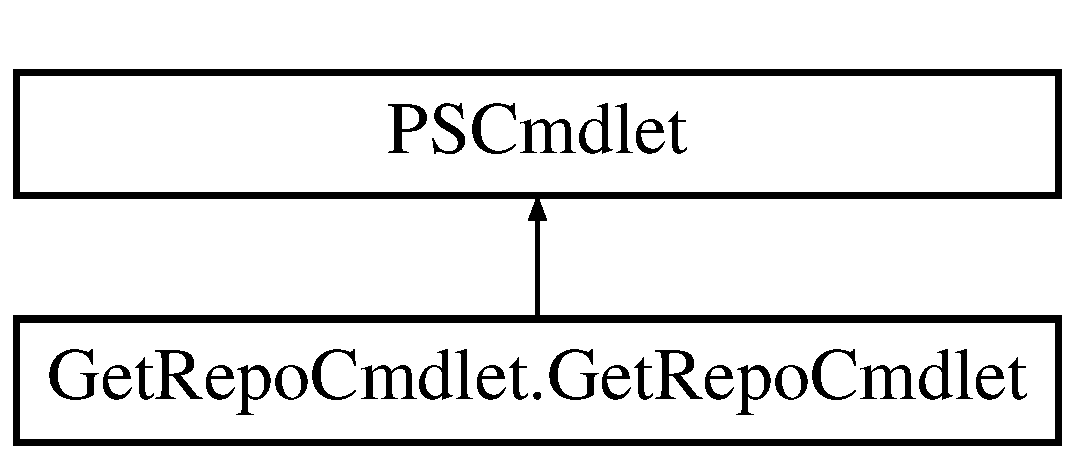
\includegraphics[height=2.000000cm]{class_get_repo_cmdlet_1_1_get_repo_cmdlet}
\end{center}
\end{figure}
\subsection*{Protected Member Functions}
\begin{DoxyCompactItemize}
\item 
override void \mbox{\hyperlink{class_get_repo_cmdlet_1_1_get_repo_cmdlet_a22503338cdb62a648a848cd8fcbf7769}{Begin\+Processing}} ()
\begin{DoxyCompactList}\small\item\em Override of the base method for \end{DoxyCompactList}\item 
override void \mbox{\hyperlink{class_get_repo_cmdlet_1_1_get_repo_cmdlet_ada76037eb2a8eed81eb1bb7a21d84693}{Process\+Record}} ()
\begin{DoxyCompactList}\small\item\em Override of the base method for \end{DoxyCompactList}\item 
override void \mbox{\hyperlink{class_get_repo_cmdlet_1_1_get_repo_cmdlet_a0968e20b2c03f033c93c2a74c643d06b}{End\+Processing}} ()
\begin{DoxyCompactList}\small\item\em Override of the base method for \end{DoxyCompactList}\end{DoxyCompactItemize}
\subsection*{Properties}
\begin{DoxyCompactItemize}
\item 
string \mbox{\hyperlink{class_get_repo_cmdlet_1_1_get_repo_cmdlet_ab8b0954fb74d52faa018ff0b721f7291}{Git\+Repo}}\hspace{0.3cm}{\ttfamily  \mbox{[}get, set\mbox{]}}
\begin{DoxyCompactList}\small\item\em Accepts the mandatory parameter to declare the git repo. Accepts both a properly formed U\+RL to a git repo, or a repo name that is a part of the Great\+America collection. \end{DoxyCompactList}\item 
string \mbox{\hyperlink{class_get_repo_cmdlet_1_1_get_repo_cmdlet_ac98a9c9f16239f0dfd0d3649a79a66e5}{Branch}}\hspace{0.3cm}{\ttfamily  \mbox{[}get, set\mbox{]}}
\begin{DoxyCompactList}\small\item\em Defines a specific branch to clone. Must be a pre-\/existing branch. \end{DoxyCompactList}\item 
Switch\+Parameter \mbox{\hyperlink{class_get_repo_cmdlet_1_1_get_repo_cmdlet_a11300c987e6547a3282664b6ff3c02d3}{Stop\+Execute}}\hspace{0.3cm}{\ttfamily  \mbox{[}get, set\mbox{]}}
\begin{DoxyCompactList}\small\item\em Parameter flag that stops execution after git command. \end{DoxyCompactList}\item 
double \mbox{\hyperlink{class_get_repo_cmdlet_1_1_get_repo_cmdlet_a0fb47dd1e2551b3883abaacf1c94057c}{V\+S\+Version}}\hspace{0.3cm}{\ttfamily  \mbox{[}get, set\mbox{]}}
\begin{DoxyCompactList}\small\item\em Parameter that collects the version/year of the VS to be used in launching the program. \end{DoxyCompactList}\item 
Switch\+Parameter \mbox{\hyperlink{class_get_repo_cmdlet_1_1_get_repo_cmdlet_a9e8a15001d9ad8bc691ebfb75a7a5993}{Exit}}\hspace{0.3cm}{\ttfamily  \mbox{[}get, set\mbox{]}}
\begin{DoxyCompactList}\small\item\em Parameter flag that closes the PS instance after completing processing. \end{DoxyCompactList}\end{DoxyCompactItemize}
\subsection*{Private Member Functions}
\begin{DoxyCompactItemize}
\item 
void \mbox{\hyperlink{class_get_repo_cmdlet_1_1_get_repo_cmdlet_a6d4524a1c3d700585b10ba0f0a6ec157}{Execute\+Git}} ()
\begin{DoxyCompactList}\small\item\em Executes and completes execution of necessary git commands. Process is created to run in parallel, and uses async calls to print execution messages back to the invoking PS instance. \end{DoxyCompactList}\item 
void \mbox{\hyperlink{class_get_repo_cmdlet_1_1_get_repo_cmdlet_afe285942efc86534f71f64c78fbb2445}{Write\+Fail\+Message}} (string message)
\begin{DoxyCompactList}\small\item\em Writes the passed failure message to the cmd prompt. \end{DoxyCompactList}\item 
void \mbox{\hyperlink{class_get_repo_cmdlet_1_1_get_repo_cmdlet_abd3278e2a9e0b1a3ac95dfee3eeb6bdc}{Write\+Warning\+Message}} (string message)
\begin{DoxyCompactList}\small\item\em Writes the passed warning message to cmd prompt. \end{DoxyCompactList}\item 
void \mbox{\hyperlink{class_get_repo_cmdlet_1_1_get_repo_cmdlet_aabc925069bb0855f2cd1e07ae832b44a}{Write\+Information\+Message}} (string message)
\begin{DoxyCompactList}\small\item\em Writes the passed information message to cmd prompt. \end{DoxyCompactList}\end{DoxyCompactItemize}
\subsection*{Private Attributes}
\begin{DoxyCompactItemize}
\item 
\mbox{\hyperlink{class_get_repo_cmdlet_1_1_cmd_container}{Cmd\+Container}} \mbox{\hyperlink{class_get_repo_cmdlet_1_1_get_repo_cmdlet_a822f61308706124cb1f17d9cd1af1092}{\+\_\+cmd\+Container}}
\begin{DoxyCompactList}\small\item\em Instance variable to hold parameters and processing information. \end{DoxyCompactList}\end{DoxyCompactItemize}


\subsection{Detailed Description}
Cmdlet definition class to create Get-\/\+Repo cmdlet. 



Definition at line 15 of file Get\+Repo\+Cmdlet.\+cs.



\subsection{Member Function Documentation}
\mbox{\Hypertarget{class_get_repo_cmdlet_1_1_get_repo_cmdlet_a22503338cdb62a648a848cd8fcbf7769}\label{class_get_repo_cmdlet_1_1_get_repo_cmdlet_a22503338cdb62a648a848cd8fcbf7769}} 
\index{Get\+Repo\+Cmdlet\+::\+Get\+Repo\+Cmdlet@{Get\+Repo\+Cmdlet\+::\+Get\+Repo\+Cmdlet}!Begin\+Processing@{Begin\+Processing}}
\index{Begin\+Processing@{Begin\+Processing}!Get\+Repo\+Cmdlet\+::\+Get\+Repo\+Cmdlet@{Get\+Repo\+Cmdlet\+::\+Get\+Repo\+Cmdlet}}
\subsubsection{\texorpdfstring{Begin\+Processing()}{BeginProcessing()}}
{\footnotesize\ttfamily override void Get\+Repo\+Cmdlet.\+Get\+Repo\+Cmdlet.\+Begin\+Processing (\begin{DoxyParamCaption}{ }\end{DoxyParamCaption})\hspace{0.3cm}{\ttfamily [protected]}}



Override of the base method for 

{\ttfamily \mbox{\hyperlink{class_get_repo_cmdlet_1_1_get_repo_cmdlet_a22503338cdb62a648a848cd8fcbf7769}{Begin\+Processing()}}}. This override method handles instantiation and preparation of the passed information in the command. 


\begin{DoxyExceptions}{Exceptions}
{\em \mbox{\hyperlink{class_get_repo_cmdlet_1_1_invalid_git_repo_exception}{Invalid\+Git\+Repo\+Exception}}} & Invalid git parameter entry will trigger this exception and halt the command. \\
\hline
\end{DoxyExceptions}
\begin{DoxySeeAlso}{See also}
Git\+Param\+Type, \mbox{\hyperlink{class_get_repo_cmdlet_1_1_processor_a0fba012ba15720a0fcd419c44b757c5b}{Processor.\+Validate\+Git\+Param(string)}}, \mbox{\hyperlink{class_get_repo_cmdlet_1_1_cmd_container}{Cmd\+Container}}


\end{DoxySeeAlso}


Definition at line 95 of file Get\+Repo\+Cmdlet.\+cs.

\mbox{\Hypertarget{class_get_repo_cmdlet_1_1_get_repo_cmdlet_a0968e20b2c03f033c93c2a74c643d06b}\label{class_get_repo_cmdlet_1_1_get_repo_cmdlet_a0968e20b2c03f033c93c2a74c643d06b}} 
\index{Get\+Repo\+Cmdlet\+::\+Get\+Repo\+Cmdlet@{Get\+Repo\+Cmdlet\+::\+Get\+Repo\+Cmdlet}!End\+Processing@{End\+Processing}}
\index{End\+Processing@{End\+Processing}!Get\+Repo\+Cmdlet\+::\+Get\+Repo\+Cmdlet@{Get\+Repo\+Cmdlet\+::\+Get\+Repo\+Cmdlet}}
\subsubsection{\texorpdfstring{End\+Processing()}{EndProcessing()}}
{\footnotesize\ttfamily override void Get\+Repo\+Cmdlet.\+Get\+Repo\+Cmdlet.\+End\+Processing (\begin{DoxyParamCaption}{ }\end{DoxyParamCaption})\hspace{0.3cm}{\ttfamily [protected]}}



Override of the base method for 

{\ttfamily \mbox{\hyperlink{class_get_repo_cmdlet_1_1_get_repo_cmdlet_a0968e20b2c03f033c93c2a74c643d06b}{End\+Processing()}}}. Handles closeout logic, and how to handle the PS command window instance. 

\begin{DoxySeeAlso}{See also}
\mbox{\hyperlink{class_get_repo_cmdlet_1_1_cmd_container}{Cmd\+Container}}


\end{DoxySeeAlso}


Definition at line 189 of file Get\+Repo\+Cmdlet.\+cs.

\mbox{\Hypertarget{class_get_repo_cmdlet_1_1_get_repo_cmdlet_a6d4524a1c3d700585b10ba0f0a6ec157}\label{class_get_repo_cmdlet_1_1_get_repo_cmdlet_a6d4524a1c3d700585b10ba0f0a6ec157}} 
\index{Get\+Repo\+Cmdlet\+::\+Get\+Repo\+Cmdlet@{Get\+Repo\+Cmdlet\+::\+Get\+Repo\+Cmdlet}!Execute\+Git@{Execute\+Git}}
\index{Execute\+Git@{Execute\+Git}!Get\+Repo\+Cmdlet\+::\+Get\+Repo\+Cmdlet@{Get\+Repo\+Cmdlet\+::\+Get\+Repo\+Cmdlet}}
\subsubsection{\texorpdfstring{Execute\+Git()}{ExecuteGit()}}
{\footnotesize\ttfamily void Get\+Repo\+Cmdlet.\+Get\+Repo\+Cmdlet.\+Execute\+Git (\begin{DoxyParamCaption}{ }\end{DoxyParamCaption})\hspace{0.3cm}{\ttfamily [private]}}



Executes and completes execution of necessary git commands. Process is created to run in parallel, and uses async calls to print execution messages back to the invoking PS instance. 



Definition at line 204 of file Get\+Repo\+Cmdlet.\+cs.

\mbox{\Hypertarget{class_get_repo_cmdlet_1_1_get_repo_cmdlet_ada76037eb2a8eed81eb1bb7a21d84693}\label{class_get_repo_cmdlet_1_1_get_repo_cmdlet_ada76037eb2a8eed81eb1bb7a21d84693}} 
\index{Get\+Repo\+Cmdlet\+::\+Get\+Repo\+Cmdlet@{Get\+Repo\+Cmdlet\+::\+Get\+Repo\+Cmdlet}!Process\+Record@{Process\+Record}}
\index{Process\+Record@{Process\+Record}!Get\+Repo\+Cmdlet\+::\+Get\+Repo\+Cmdlet@{Get\+Repo\+Cmdlet\+::\+Get\+Repo\+Cmdlet}}
\subsubsection{\texorpdfstring{Process\+Record()}{ProcessRecord()}}
{\footnotesize\ttfamily override void Get\+Repo\+Cmdlet.\+Get\+Repo\+Cmdlet.\+Process\+Record (\begin{DoxyParamCaption}{ }\end{DoxyParamCaption})\hspace{0.3cm}{\ttfamily [protected]}}



Override of the base method for 

{\ttfamily \mbox{\hyperlink{class_get_repo_cmdlet_1_1_get_repo_cmdlet_ada76037eb2a8eed81eb1bb7a21d84693}{Process\+Record()}}}. This override method handles delegating all processing work to the \mbox{\hyperlink{class_get_repo_cmdlet_1_1_processor}{Processor}} class. 

\begin{DoxySeeAlso}{See also}
\mbox{\hyperlink{class_get_repo_cmdlet_1_1_processor_ace9c1d574b3758f94c8cf65e7fcddbf3}{Processor.\+Check\+For\+Existing\+Directory(string)}}, Processor.\+Backup\+Directory(string, string, string), \mbox{\hyperlink{class_get_repo_cmdlet_1_1_processor_ae5f7bb67f8595174379a2cb144ae22c3}{Processor.\+Delete\+Directory(string)}}, \mbox{\hyperlink{class_get_repo_cmdlet_1_1_processor_a9c532782d2575d5244440407103b4352}{Processor.\+Prepare\+Git\+Cmd(\+Git\+Command, string, string)}}, \mbox{\hyperlink{class_get_repo_cmdlet_1_1_processor_a0d3e38fbd41a8e6bdfbc62dcf4656e90}{Processor.\+Launch\+V\+S(\+Cmd\+Container)}}, \mbox{\hyperlink{class_get_repo_cmdlet_1_1_cmd_container}{Cmd\+Container}}


\end{DoxySeeAlso}


Definition at line 131 of file Get\+Repo\+Cmdlet.\+cs.

\mbox{\Hypertarget{class_get_repo_cmdlet_1_1_get_repo_cmdlet_afe285942efc86534f71f64c78fbb2445}\label{class_get_repo_cmdlet_1_1_get_repo_cmdlet_afe285942efc86534f71f64c78fbb2445}} 
\index{Get\+Repo\+Cmdlet\+::\+Get\+Repo\+Cmdlet@{Get\+Repo\+Cmdlet\+::\+Get\+Repo\+Cmdlet}!Write\+Fail\+Message@{Write\+Fail\+Message}}
\index{Write\+Fail\+Message@{Write\+Fail\+Message}!Get\+Repo\+Cmdlet\+::\+Get\+Repo\+Cmdlet@{Get\+Repo\+Cmdlet\+::\+Get\+Repo\+Cmdlet}}
\subsubsection{\texorpdfstring{Write\+Fail\+Message()}{WriteFailMessage()}}
{\footnotesize\ttfamily void Get\+Repo\+Cmdlet.\+Get\+Repo\+Cmdlet.\+Write\+Fail\+Message (\begin{DoxyParamCaption}\item[{string}]{message }\end{DoxyParamCaption})\hspace{0.3cm}{\ttfamily [private]}}



Writes the passed failure message to the cmd prompt. 


\begin{DoxyParams}{Parameters}
{\em message} & The message.\\
\hline
\end{DoxyParams}


Definition at line 253 of file Get\+Repo\+Cmdlet.\+cs.

\mbox{\Hypertarget{class_get_repo_cmdlet_1_1_get_repo_cmdlet_aabc925069bb0855f2cd1e07ae832b44a}\label{class_get_repo_cmdlet_1_1_get_repo_cmdlet_aabc925069bb0855f2cd1e07ae832b44a}} 
\index{Get\+Repo\+Cmdlet\+::\+Get\+Repo\+Cmdlet@{Get\+Repo\+Cmdlet\+::\+Get\+Repo\+Cmdlet}!Write\+Information\+Message@{Write\+Information\+Message}}
\index{Write\+Information\+Message@{Write\+Information\+Message}!Get\+Repo\+Cmdlet\+::\+Get\+Repo\+Cmdlet@{Get\+Repo\+Cmdlet\+::\+Get\+Repo\+Cmdlet}}
\subsubsection{\texorpdfstring{Write\+Information\+Message()}{WriteInformationMessage()}}
{\footnotesize\ttfamily void Get\+Repo\+Cmdlet.\+Get\+Repo\+Cmdlet.\+Write\+Information\+Message (\begin{DoxyParamCaption}\item[{string}]{message }\end{DoxyParamCaption})\hspace{0.3cm}{\ttfamily [private]}}



Writes the passed information message to cmd prompt. 


\begin{DoxyParams}{Parameters}
{\em message} & The message.\\
\hline
\end{DoxyParams}


Definition at line 271 of file Get\+Repo\+Cmdlet.\+cs.

\mbox{\Hypertarget{class_get_repo_cmdlet_1_1_get_repo_cmdlet_abd3278e2a9e0b1a3ac95dfee3eeb6bdc}\label{class_get_repo_cmdlet_1_1_get_repo_cmdlet_abd3278e2a9e0b1a3ac95dfee3eeb6bdc}} 
\index{Get\+Repo\+Cmdlet\+::\+Get\+Repo\+Cmdlet@{Get\+Repo\+Cmdlet\+::\+Get\+Repo\+Cmdlet}!Write\+Warning\+Message@{Write\+Warning\+Message}}
\index{Write\+Warning\+Message@{Write\+Warning\+Message}!Get\+Repo\+Cmdlet\+::\+Get\+Repo\+Cmdlet@{Get\+Repo\+Cmdlet\+::\+Get\+Repo\+Cmdlet}}
\subsubsection{\texorpdfstring{Write\+Warning\+Message()}{WriteWarningMessage()}}
{\footnotesize\ttfamily void Get\+Repo\+Cmdlet.\+Get\+Repo\+Cmdlet.\+Write\+Warning\+Message (\begin{DoxyParamCaption}\item[{string}]{message }\end{DoxyParamCaption})\hspace{0.3cm}{\ttfamily [private]}}



Writes the passed warning message to cmd prompt. 


\begin{DoxyParams}{Parameters}
{\em message} & The message.\\
\hline
\end{DoxyParams}


Definition at line 262 of file Get\+Repo\+Cmdlet.\+cs.



\subsection{Member Data Documentation}
\mbox{\Hypertarget{class_get_repo_cmdlet_1_1_get_repo_cmdlet_a822f61308706124cb1f17d9cd1af1092}\label{class_get_repo_cmdlet_1_1_get_repo_cmdlet_a822f61308706124cb1f17d9cd1af1092}} 
\index{Get\+Repo\+Cmdlet\+::\+Get\+Repo\+Cmdlet@{Get\+Repo\+Cmdlet\+::\+Get\+Repo\+Cmdlet}!\+\_\+cmd\+Container@{\+\_\+cmd\+Container}}
\index{\+\_\+cmd\+Container@{\+\_\+cmd\+Container}!Get\+Repo\+Cmdlet\+::\+Get\+Repo\+Cmdlet@{Get\+Repo\+Cmdlet\+::\+Get\+Repo\+Cmdlet}}
\subsubsection{\texorpdfstring{\+\_\+cmd\+Container}{\_cmdContainer}}
{\footnotesize\ttfamily \mbox{\hyperlink{class_get_repo_cmdlet_1_1_cmd_container}{Cmd\+Container}} Get\+Repo\+Cmdlet.\+Get\+Repo\+Cmdlet.\+\_\+cmd\+Container\hspace{0.3cm}{\ttfamily [private]}}



Instance variable to hold parameters and processing information. 



Definition at line 80 of file Get\+Repo\+Cmdlet.\+cs.



\subsection{Property Documentation}
\mbox{\Hypertarget{class_get_repo_cmdlet_1_1_get_repo_cmdlet_ac98a9c9f16239f0dfd0d3649a79a66e5}\label{class_get_repo_cmdlet_1_1_get_repo_cmdlet_ac98a9c9f16239f0dfd0d3649a79a66e5}} 
\index{Get\+Repo\+Cmdlet\+::\+Get\+Repo\+Cmdlet@{Get\+Repo\+Cmdlet\+::\+Get\+Repo\+Cmdlet}!Branch@{Branch}}
\index{Branch@{Branch}!Get\+Repo\+Cmdlet\+::\+Get\+Repo\+Cmdlet@{Get\+Repo\+Cmdlet\+::\+Get\+Repo\+Cmdlet}}
\subsubsection{\texorpdfstring{Branch}{Branch}}
{\footnotesize\ttfamily string Get\+Repo\+Cmdlet.\+Get\+Repo\+Cmdlet.\+Branch\hspace{0.3cm}{\ttfamily [get]}, {\ttfamily [set]}}



Defines a specific branch to clone. Must be a pre-\/existing branch. 

To clone the branch \char`\"{}\+My\+Branch\char`\"{}\+: Get-\/\+Repo \href{https://github.com/Greatamerica/MyRepo}{\tt https\+://github.\+com/\+Greatamerica/\+My\+Repo} -\/\+Branch My\+Branch 

Definition at line 41 of file Get\+Repo\+Cmdlet.\+cs.

\mbox{\Hypertarget{class_get_repo_cmdlet_1_1_get_repo_cmdlet_a9e8a15001d9ad8bc691ebfb75a7a5993}\label{class_get_repo_cmdlet_1_1_get_repo_cmdlet_a9e8a15001d9ad8bc691ebfb75a7a5993}} 
\index{Get\+Repo\+Cmdlet\+::\+Get\+Repo\+Cmdlet@{Get\+Repo\+Cmdlet\+::\+Get\+Repo\+Cmdlet}!Exit@{Exit}}
\index{Exit@{Exit}!Get\+Repo\+Cmdlet\+::\+Get\+Repo\+Cmdlet@{Get\+Repo\+Cmdlet\+::\+Get\+Repo\+Cmdlet}}
\subsubsection{\texorpdfstring{Exit}{Exit}}
{\footnotesize\ttfamily Switch\+Parameter Get\+Repo\+Cmdlet.\+Get\+Repo\+Cmdlet.\+Exit\hspace{0.3cm}{\ttfamily [get]}, {\ttfamily [set]}}



Parameter flag that closes the PS instance after completing processing. 



Definition at line 75 of file Get\+Repo\+Cmdlet.\+cs.

\mbox{\Hypertarget{class_get_repo_cmdlet_1_1_get_repo_cmdlet_ab8b0954fb74d52faa018ff0b721f7291}\label{class_get_repo_cmdlet_1_1_get_repo_cmdlet_ab8b0954fb74d52faa018ff0b721f7291}} 
\index{Get\+Repo\+Cmdlet\+::\+Get\+Repo\+Cmdlet@{Get\+Repo\+Cmdlet\+::\+Get\+Repo\+Cmdlet}!Git\+Repo@{Git\+Repo}}
\index{Git\+Repo@{Git\+Repo}!Get\+Repo\+Cmdlet\+::\+Get\+Repo\+Cmdlet@{Get\+Repo\+Cmdlet\+::\+Get\+Repo\+Cmdlet}}
\subsubsection{\texorpdfstring{Git\+Repo}{GitRepo}}
{\footnotesize\ttfamily string Get\+Repo\+Cmdlet.\+Get\+Repo\+Cmdlet.\+Git\+Repo\hspace{0.3cm}{\ttfamily [get]}, {\ttfamily [set]}}



Accepts the mandatory parameter to declare the git repo. Accepts both a properly formed U\+RL to a git repo, or a repo name that is a part of the Great\+America collection. 

Both of these examples will result in cloning the same repo (\char`\"{}\+My\+Repo\char`\"{})\+: U\+RL entry\+: Get-\/\+Repo \href{https://github.com/GreatAmerica/MyRepo}{\tt https\+://github.\+com/\+Great\+America/\+My\+Repo} Repo entry\+: Get-\/\+Repo My\+Repo 

Definition at line 30 of file Get\+Repo\+Cmdlet.\+cs.

\mbox{\Hypertarget{class_get_repo_cmdlet_1_1_get_repo_cmdlet_a11300c987e6547a3282664b6ff3c02d3}\label{class_get_repo_cmdlet_1_1_get_repo_cmdlet_a11300c987e6547a3282664b6ff3c02d3}} 
\index{Get\+Repo\+Cmdlet\+::\+Get\+Repo\+Cmdlet@{Get\+Repo\+Cmdlet\+::\+Get\+Repo\+Cmdlet}!Stop\+Execute@{Stop\+Execute}}
\index{Stop\+Execute@{Stop\+Execute}!Get\+Repo\+Cmdlet\+::\+Get\+Repo\+Cmdlet@{Get\+Repo\+Cmdlet\+::\+Get\+Repo\+Cmdlet}}
\subsubsection{\texorpdfstring{Stop\+Execute}{StopExecute}}
{\footnotesize\ttfamily Switch\+Parameter Get\+Repo\+Cmdlet.\+Get\+Repo\+Cmdlet.\+Stop\+Execute\hspace{0.3cm}{\ttfamily [get]}, {\ttfamily [set]}}



Parameter flag that stops execution after git command. 

This parameter takes precedence over V\+S\+Version.

Both of these result in preventing the solution from opening\+: Get-\/\+Repo \href{https://github.com/Greatamerica/MyRepo}{\tt https\+://github.\+com/\+Greatamerica/\+My\+Repo} -\/\+Stop\+Execute Get-\/\+Repo \href{https://github.com/Greatamerica/MyRepo}{\tt https\+://github.\+com/\+Greatamerica/\+My\+Repo} -\/\+Stop\+Execute -\/\+V\+S\+Version 2017 

Definition at line 55 of file Get\+Repo\+Cmdlet.\+cs.

\mbox{\Hypertarget{class_get_repo_cmdlet_1_1_get_repo_cmdlet_a0fb47dd1e2551b3883abaacf1c94057c}\label{class_get_repo_cmdlet_1_1_get_repo_cmdlet_a0fb47dd1e2551b3883abaacf1c94057c}} 
\index{Get\+Repo\+Cmdlet\+::\+Get\+Repo\+Cmdlet@{Get\+Repo\+Cmdlet\+::\+Get\+Repo\+Cmdlet}!V\+S\+Version@{V\+S\+Version}}
\index{V\+S\+Version@{V\+S\+Version}!Get\+Repo\+Cmdlet\+::\+Get\+Repo\+Cmdlet@{Get\+Repo\+Cmdlet\+::\+Get\+Repo\+Cmdlet}}
\subsubsection{\texorpdfstring{V\+S\+Version}{VSVersion}}
{\footnotesize\ttfamily double Get\+Repo\+Cmdlet.\+Get\+Repo\+Cmdlet.\+V\+S\+Version\hspace{0.3cm}{\ttfamily [get]}, {\ttfamily [set]}}



Parameter that collects the version/year of the VS to be used in launching the program. 

If this parameter and the Stop\+Execute flag are both present, Stop\+Execute takes precedence over V\+S\+Version and will halt execution. 

Definition at line 68 of file Get\+Repo\+Cmdlet.\+cs.



The documentation for this class was generated from the following file\+:\begin{DoxyCompactItemize}
\item 
Get\+Repo\+Cmdlet/\mbox{\hyperlink{_get_repo_cmdlet_8cs}{Get\+Repo\+Cmdlet.\+cs}}\end{DoxyCompactItemize}

\hypertarget{class_get_repo_cmdlet_1_1_invalid_git_repo_exception}{}\section{Get\+Repo\+Cmdlet.\+Invalid\+Git\+Repo\+Exception Class Reference}
\label{class_get_repo_cmdlet_1_1_invalid_git_repo_exception}\index{Get\+Repo\+Cmdlet.\+Invalid\+Git\+Repo\+Exception@{Get\+Repo\+Cmdlet.\+Invalid\+Git\+Repo\+Exception}}


Custom application exception to handle invalid entries in the Git\+Repo parameter.  


Inheritance diagram for Get\+Repo\+Cmdlet.\+Invalid\+Git\+Repo\+Exception\+:\begin{figure}[H]
\begin{center}
\leavevmode
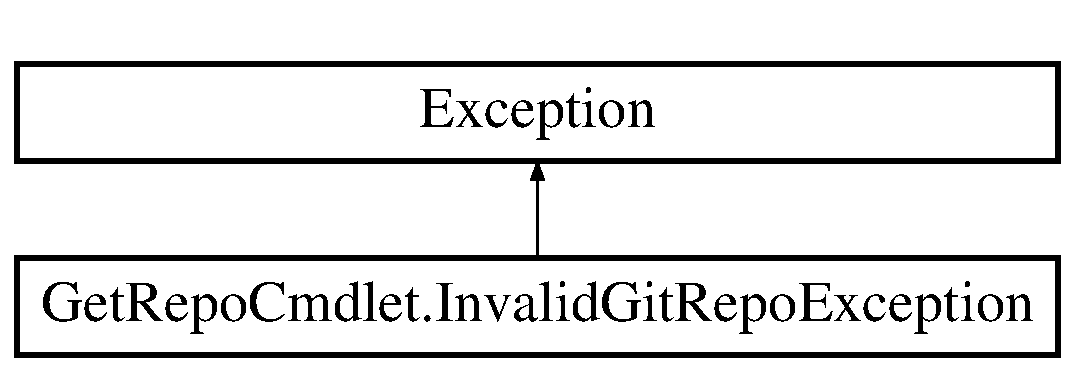
\includegraphics[height=2.000000cm]{class_get_repo_cmdlet_1_1_invalid_git_repo_exception}
\end{center}
\end{figure}
\subsection*{Public Member Functions}
\begin{DoxyCompactItemize}
\item 
\mbox{\hyperlink{class_get_repo_cmdlet_1_1_invalid_git_repo_exception_a806265e644c40f10548f065775b3ff6f}{Invalid\+Git\+Repo\+Exception}} ()
\begin{DoxyCompactList}\small\item\em Initializes a new instance of the \mbox{\hyperlink{class_get_repo_cmdlet_1_1_invalid_git_repo_exception}{Invalid\+Git\+Repo\+Exception}} class. \end{DoxyCompactList}\item 
\mbox{\hyperlink{class_get_repo_cmdlet_1_1_invalid_git_repo_exception_a14241ad466219ffb1c58e0e558397736}{Invalid\+Git\+Repo\+Exception}} (string message)
\begin{DoxyCompactList}\small\item\em Initializes a new instance of the \mbox{\hyperlink{class_get_repo_cmdlet_1_1_invalid_git_repo_exception}{Invalid\+Git\+Repo\+Exception}} class. \end{DoxyCompactList}\item 
\mbox{\hyperlink{class_get_repo_cmdlet_1_1_invalid_git_repo_exception_a7c08597e5771ae9c41171ddc486b746f}{Invalid\+Git\+Repo\+Exception}} (string message, System.\+Exception inner)
\begin{DoxyCompactList}\small\item\em Initializes a new instance of the \mbox{\hyperlink{class_get_repo_cmdlet_1_1_invalid_git_repo_exception}{Invalid\+Git\+Repo\+Exception}} class. \end{DoxyCompactList}\end{DoxyCompactItemize}


\subsection{Detailed Description}
Custom application exception to handle invalid entries in the Git\+Repo parameter. 

\begin{DoxySeeAlso}{See also}
System.\+Exception


\end{DoxySeeAlso}


Definition at line 160 of file Get\+Repo\+Cmdlet.\+Objects.\+cs.



\subsection{Constructor \& Destructor Documentation}
\mbox{\Hypertarget{class_get_repo_cmdlet_1_1_invalid_git_repo_exception_a806265e644c40f10548f065775b3ff6f}\label{class_get_repo_cmdlet_1_1_invalid_git_repo_exception_a806265e644c40f10548f065775b3ff6f}} 
\index{Get\+Repo\+Cmdlet\+::\+Invalid\+Git\+Repo\+Exception@{Get\+Repo\+Cmdlet\+::\+Invalid\+Git\+Repo\+Exception}!Invalid\+Git\+Repo\+Exception@{Invalid\+Git\+Repo\+Exception}}
\index{Invalid\+Git\+Repo\+Exception@{Invalid\+Git\+Repo\+Exception}!Get\+Repo\+Cmdlet\+::\+Invalid\+Git\+Repo\+Exception@{Get\+Repo\+Cmdlet\+::\+Invalid\+Git\+Repo\+Exception}}
\subsubsection{\texorpdfstring{Invalid\+Git\+Repo\+Exception()}{InvalidGitRepoException()}\hspace{0.1cm}{\footnotesize\ttfamily [1/3]}}
{\footnotesize\ttfamily Get\+Repo\+Cmdlet.\+Invalid\+Git\+Repo\+Exception.\+Invalid\+Git\+Repo\+Exception (\begin{DoxyParamCaption}{ }\end{DoxyParamCaption})}



Initializes a new instance of the \mbox{\hyperlink{class_get_repo_cmdlet_1_1_invalid_git_repo_exception}{Invalid\+Git\+Repo\+Exception}} class. 

\begin{DoxySeeAlso}{See also}
\mbox{\hyperlink{class_get_repo_cmdlet_1_1_const_mgr_a84baefdb7fb1bcd31e0148b4ce532d8f}{Const\+Mgr.\+Invalid\+Git\+Repo\+Exception\+Message}}


\end{DoxySeeAlso}


Definition at line 166 of file Get\+Repo\+Cmdlet.\+Objects.\+cs.

\mbox{\Hypertarget{class_get_repo_cmdlet_1_1_invalid_git_repo_exception_a14241ad466219ffb1c58e0e558397736}\label{class_get_repo_cmdlet_1_1_invalid_git_repo_exception_a14241ad466219ffb1c58e0e558397736}} 
\index{Get\+Repo\+Cmdlet\+::\+Invalid\+Git\+Repo\+Exception@{Get\+Repo\+Cmdlet\+::\+Invalid\+Git\+Repo\+Exception}!Invalid\+Git\+Repo\+Exception@{Invalid\+Git\+Repo\+Exception}}
\index{Invalid\+Git\+Repo\+Exception@{Invalid\+Git\+Repo\+Exception}!Get\+Repo\+Cmdlet\+::\+Invalid\+Git\+Repo\+Exception@{Get\+Repo\+Cmdlet\+::\+Invalid\+Git\+Repo\+Exception}}
\subsubsection{\texorpdfstring{Invalid\+Git\+Repo\+Exception()}{InvalidGitRepoException()}\hspace{0.1cm}{\footnotesize\ttfamily [2/3]}}
{\footnotesize\ttfamily Get\+Repo\+Cmdlet.\+Invalid\+Git\+Repo\+Exception.\+Invalid\+Git\+Repo\+Exception (\begin{DoxyParamCaption}\item[{string}]{message }\end{DoxyParamCaption})}



Initializes a new instance of the \mbox{\hyperlink{class_get_repo_cmdlet_1_1_invalid_git_repo_exception}{Invalid\+Git\+Repo\+Exception}} class. 


\begin{DoxyParams}{Parameters}
{\em message} & The message that describes the error.\\
\hline
\end{DoxyParams}
\begin{DoxySeeAlso}{See also}
\mbox{\hyperlink{class_get_repo_cmdlet_1_1_const_mgr_a84baefdb7fb1bcd31e0148b4ce532d8f}{Const\+Mgr.\+Invalid\+Git\+Repo\+Exception\+Message}}


\end{DoxySeeAlso}


Definition at line 175 of file Get\+Repo\+Cmdlet.\+Objects.\+cs.

\mbox{\Hypertarget{class_get_repo_cmdlet_1_1_invalid_git_repo_exception_a7c08597e5771ae9c41171ddc486b746f}\label{class_get_repo_cmdlet_1_1_invalid_git_repo_exception_a7c08597e5771ae9c41171ddc486b746f}} 
\index{Get\+Repo\+Cmdlet\+::\+Invalid\+Git\+Repo\+Exception@{Get\+Repo\+Cmdlet\+::\+Invalid\+Git\+Repo\+Exception}!Invalid\+Git\+Repo\+Exception@{Invalid\+Git\+Repo\+Exception}}
\index{Invalid\+Git\+Repo\+Exception@{Invalid\+Git\+Repo\+Exception}!Get\+Repo\+Cmdlet\+::\+Invalid\+Git\+Repo\+Exception@{Get\+Repo\+Cmdlet\+::\+Invalid\+Git\+Repo\+Exception}}
\subsubsection{\texorpdfstring{Invalid\+Git\+Repo\+Exception()}{InvalidGitRepoException()}\hspace{0.1cm}{\footnotesize\ttfamily [3/3]}}
{\footnotesize\ttfamily Get\+Repo\+Cmdlet.\+Invalid\+Git\+Repo\+Exception.\+Invalid\+Git\+Repo\+Exception (\begin{DoxyParamCaption}\item[{string}]{message,  }\item[{System.\+Exception}]{inner }\end{DoxyParamCaption})}



Initializes a new instance of the \mbox{\hyperlink{class_get_repo_cmdlet_1_1_invalid_git_repo_exception}{Invalid\+Git\+Repo\+Exception}} class. 


\begin{DoxyParams}{Parameters}
{\em message} & The message that describes the error.\\
\hline
{\em inner} & The inner exception.\\
\hline
\end{DoxyParams}
\begin{DoxySeeAlso}{See also}
\mbox{\hyperlink{class_get_repo_cmdlet_1_1_const_mgr_a84baefdb7fb1bcd31e0148b4ce532d8f}{Const\+Mgr.\+Invalid\+Git\+Repo\+Exception\+Message}}


\end{DoxySeeAlso}


Definition at line 185 of file Get\+Repo\+Cmdlet.\+Objects.\+cs.



The documentation for this class was generated from the following file\+:\begin{DoxyCompactItemize}
\item 
Get\+Repo\+Cmdlet/\mbox{\hyperlink{_get_repo_cmdlet_8_objects_8cs}{Get\+Repo\+Cmdlet.\+Objects.\+cs}}\end{DoxyCompactItemize}

\hypertarget{class_get_repo_cmdlet_1_1_processor}{}\section{Get\+Repo\+Cmdlet.\+Processor Class Reference}
\label{class_get_repo_cmdlet_1_1_processor}\index{Get\+Repo\+Cmdlet.\+Processor@{Get\+Repo\+Cmdlet.\+Processor}}


Internal static class that holds logic for execution of the cmdlet.  


\subsection*{Static Package Functions}
\begin{DoxyCompactItemize}
\item 
static Git\+Param\+Type \mbox{\hyperlink{class_get_repo_cmdlet_1_1_processor_a0fba012ba15720a0fcd419c44b757c5b}{Validate\+Git\+Param}} (string git\+Param)
\begin{DoxyCompactList}\small\item\em Validates the git parameter based on a regex expression to determine both validity, as well as if it is a U\+RL or repo name. \end{DoxyCompactList}\item 
static string \mbox{\hyperlink{class_get_repo_cmdlet_1_1_processor_a9c532782d2575d5244440407103b4352}{Prepare\+Git\+Cmd}} (Git\+Command git\+Cmd, string repo\+U\+RL, string branch)
\begin{DoxyCompactList}\small\item\em Prepares the git command. \end{DoxyCompactList}\item 
static string \mbox{\hyperlink{class_get_repo_cmdlet_1_1_processor_a4a96e92b1c20e4f4fc38f9230d51912a}{Create\+Repo\+Name}} (string git\+Repo\+\_\+\+U\+RL)
\begin{DoxyCompactList}\small\item\em Creates the name of the repo from the U\+RL passed. \end{DoxyCompactList}\item 
static string \mbox{\hyperlink{class_get_repo_cmdlet_1_1_processor_ae8b0a813f91987946bfc8e218b3ab396}{Create\+Repo\+U\+RL}} (string git\+Repo\+\_\+\+N\+A\+ME)
\begin{DoxyCompactList}\small\item\em Creates the name of the repo from the repo name passed. \end{DoxyCompactList}\item 
static bool \mbox{\hyperlink{class_get_repo_cmdlet_1_1_processor_ace9c1d574b3758f94c8cf65e7fcddbf3}{Check\+For\+Existing\+Directory}} (string directory)
\begin{DoxyCompactList}\small\item\em Checks for an existing directory for this repo in the current location. \end{DoxyCompactList}\item 
static string \mbox{\hyperlink{class_get_repo_cmdlet_1_1_processor_ae0c9a18121e39f1ee3c183d08f7bf0b2}{Backup\+Directory}} (string repo\+Path)
\begin{DoxyCompactList}\small\item\em Performs a backup of the existing directory. \end{DoxyCompactList}\item 
static bool \mbox{\hyperlink{class_get_repo_cmdlet_1_1_processor_ae5f7bb67f8595174379a2cb144ae22c3}{Delete\+Directory}} (string repo\+Path)
\begin{DoxyCompactList}\small\item\em Deletes the directory passed to the method. \end{DoxyCompactList}\item 
static string \mbox{\hyperlink{class_get_repo_cmdlet_1_1_processor_a0d3e38fbd41a8e6bdfbc62dcf4656e90}{Launch\+VS}} (\mbox{\hyperlink{class_get_repo_cmdlet_1_1_cmd_container}{Cmd\+Container}} cmd\+Container)
\begin{DoxyCompactList}\small\item\em Launches Visual Studio. If no parameter was passed by V\+S\+Version, launches the default application. \end{DoxyCompactList}\end{DoxyCompactItemize}


\subsection{Detailed Description}
Internal static class that holds logic for execution of the cmdlet. 



Definition at line 13 of file Get\+Repo\+Cmdlet.\+Processor.\+cs.



\subsection{Member Function Documentation}
\mbox{\Hypertarget{class_get_repo_cmdlet_1_1_processor_ae0c9a18121e39f1ee3c183d08f7bf0b2}\label{class_get_repo_cmdlet_1_1_processor_ae0c9a18121e39f1ee3c183d08f7bf0b2}} 
\index{Get\+Repo\+Cmdlet\+::\+Processor@{Get\+Repo\+Cmdlet\+::\+Processor}!Backup\+Directory@{Backup\+Directory}}
\index{Backup\+Directory@{Backup\+Directory}!Get\+Repo\+Cmdlet\+::\+Processor@{Get\+Repo\+Cmdlet\+::\+Processor}}
\subsubsection{\texorpdfstring{Backup\+Directory()}{BackupDirectory()}}
{\footnotesize\ttfamily static string Get\+Repo\+Cmdlet.\+Processor.\+Backup\+Directory (\begin{DoxyParamCaption}\item[{string}]{repo\+Path }\end{DoxyParamCaption})\hspace{0.3cm}{\ttfamily [static]}, {\ttfamily [package]}}



Performs a backup of the existing directory. 


\begin{DoxyParams}{Parameters}
{\em repo\+Path} & The repo path to backup.\\
\hline
\end{DoxyParams}
\begin{DoxyReturn}{Returns}
The location of the backup created by the process.
\end{DoxyReturn}
\begin{DoxySeeAlso}{See also}
Bak\+Dir\+Append\+String, Bak\+Dir\+Append\+String\+\_\+\+Multi


\end{DoxySeeAlso}


Definition at line 128 of file Get\+Repo\+Cmdlet.\+Processor.\+cs.

\mbox{\Hypertarget{class_get_repo_cmdlet_1_1_processor_ace9c1d574b3758f94c8cf65e7fcddbf3}\label{class_get_repo_cmdlet_1_1_processor_ace9c1d574b3758f94c8cf65e7fcddbf3}} 
\index{Get\+Repo\+Cmdlet\+::\+Processor@{Get\+Repo\+Cmdlet\+::\+Processor}!Check\+For\+Existing\+Directory@{Check\+For\+Existing\+Directory}}
\index{Check\+For\+Existing\+Directory@{Check\+For\+Existing\+Directory}!Get\+Repo\+Cmdlet\+::\+Processor@{Get\+Repo\+Cmdlet\+::\+Processor}}
\subsubsection{\texorpdfstring{Check\+For\+Existing\+Directory()}{CheckForExistingDirectory()}}
{\footnotesize\ttfamily static bool Get\+Repo\+Cmdlet.\+Processor.\+Check\+For\+Existing\+Directory (\begin{DoxyParamCaption}\item[{string}]{directory }\end{DoxyParamCaption})\hspace{0.3cm}{\ttfamily [static]}, {\ttfamily [package]}}



Checks for an existing directory for this repo in the current location. 


\begin{DoxyParams}{Parameters}
{\em directory} & The directory to validate.\\
\hline
\end{DoxyParams}
\begin{DoxyReturn}{Returns}
{\ttfamily true} if the directory exists. {\ttfamily false} if the directory does not exist. 
\end{DoxyReturn}


Definition at line 116 of file Get\+Repo\+Cmdlet.\+Processor.\+cs.

\mbox{\Hypertarget{class_get_repo_cmdlet_1_1_processor_a4a96e92b1c20e4f4fc38f9230d51912a}\label{class_get_repo_cmdlet_1_1_processor_a4a96e92b1c20e4f4fc38f9230d51912a}} 
\index{Get\+Repo\+Cmdlet\+::\+Processor@{Get\+Repo\+Cmdlet\+::\+Processor}!Create\+Repo\+Name@{Create\+Repo\+Name}}
\index{Create\+Repo\+Name@{Create\+Repo\+Name}!Get\+Repo\+Cmdlet\+::\+Processor@{Get\+Repo\+Cmdlet\+::\+Processor}}
\subsubsection{\texorpdfstring{Create\+Repo\+Name()}{CreateRepoName()}}
{\footnotesize\ttfamily static string Get\+Repo\+Cmdlet.\+Processor.\+Create\+Repo\+Name (\begin{DoxyParamCaption}\item[{string}]{git\+Repo\+\_\+\+U\+RL }\end{DoxyParamCaption})\hspace{0.3cm}{\ttfamily [static]}, {\ttfamily [package]}}



Creates the name of the repo from the U\+RL passed. 


\begin{DoxyParams}{Parameters}
{\em git\+Repo\+\_\+\+U\+RL} & The git repo U\+RL.\\
\hline
\end{DoxyParams}
\begin{DoxyReturn}{Returns}
The repo name, extracted from the U\+RL.
\end{DoxyReturn}
\begin{DoxySeeAlso}{See also}
\mbox{\hyperlink{class_get_repo_cmdlet_1_1_processor_a0fba012ba15720a0fcd419c44b757c5b}{Validate\+Git\+Param(string)}}


\end{DoxySeeAlso}


Definition at line 88 of file Get\+Repo\+Cmdlet.\+Processor.\+cs.

\mbox{\Hypertarget{class_get_repo_cmdlet_1_1_processor_ae8b0a813f91987946bfc8e218b3ab396}\label{class_get_repo_cmdlet_1_1_processor_ae8b0a813f91987946bfc8e218b3ab396}} 
\index{Get\+Repo\+Cmdlet\+::\+Processor@{Get\+Repo\+Cmdlet\+::\+Processor}!Create\+Repo\+U\+RL@{Create\+Repo\+U\+RL}}
\index{Create\+Repo\+U\+RL@{Create\+Repo\+U\+RL}!Get\+Repo\+Cmdlet\+::\+Processor@{Get\+Repo\+Cmdlet\+::\+Processor}}
\subsubsection{\texorpdfstring{Create\+Repo\+U\+R\+L()}{CreateRepoURL()}}
{\footnotesize\ttfamily static string Get\+Repo\+Cmdlet.\+Processor.\+Create\+Repo\+U\+RL (\begin{DoxyParamCaption}\item[{string}]{git\+Repo\+\_\+\+N\+A\+ME }\end{DoxyParamCaption})\hspace{0.3cm}{\ttfamily [static]}, {\ttfamily [package]}}



Creates the name of the repo from the repo name passed. 


\begin{DoxyParams}{Parameters}
{\em git\+Repo\+\_\+\+N\+A\+ME} & The git repo name.\\
\hline
\end{DoxyParams}
\begin{DoxyReturn}{Returns}
The repo name, concatenated with constants to create the git U\+RL.
\end{DoxyReturn}
\begin{DoxySeeAlso}{See also}
\mbox{\hyperlink{class_get_repo_cmdlet_1_1_processor_a0fba012ba15720a0fcd419c44b757c5b}{Validate\+Git\+Param(string)}}, Git\+U\+R\+L\+Starter, Git\+U\+R\+L\+Ender


\end{DoxySeeAlso}


Definition at line 101 of file Get\+Repo\+Cmdlet.\+Processor.\+cs.

\mbox{\Hypertarget{class_get_repo_cmdlet_1_1_processor_ae5f7bb67f8595174379a2cb144ae22c3}\label{class_get_repo_cmdlet_1_1_processor_ae5f7bb67f8595174379a2cb144ae22c3}} 
\index{Get\+Repo\+Cmdlet\+::\+Processor@{Get\+Repo\+Cmdlet\+::\+Processor}!Delete\+Directory@{Delete\+Directory}}
\index{Delete\+Directory@{Delete\+Directory}!Get\+Repo\+Cmdlet\+::\+Processor@{Get\+Repo\+Cmdlet\+::\+Processor}}
\subsubsection{\texorpdfstring{Delete\+Directory()}{DeleteDirectory()}}
{\footnotesize\ttfamily static bool Get\+Repo\+Cmdlet.\+Processor.\+Delete\+Directory (\begin{DoxyParamCaption}\item[{string}]{repo\+Path }\end{DoxyParamCaption})\hspace{0.3cm}{\ttfamily [static]}, {\ttfamily [package]}}



Deletes the directory passed to the method. 


\begin{DoxyParams}{Parameters}
{\em repo\+Path} & The directory path to delete (the old repo).\\
\hline
\end{DoxyParams}


Definition at line 158 of file Get\+Repo\+Cmdlet.\+Processor.\+cs.

\mbox{\Hypertarget{class_get_repo_cmdlet_1_1_processor_a0d3e38fbd41a8e6bdfbc62dcf4656e90}\label{class_get_repo_cmdlet_1_1_processor_a0d3e38fbd41a8e6bdfbc62dcf4656e90}} 
\index{Get\+Repo\+Cmdlet\+::\+Processor@{Get\+Repo\+Cmdlet\+::\+Processor}!Launch\+VS@{Launch\+VS}}
\index{Launch\+VS@{Launch\+VS}!Get\+Repo\+Cmdlet\+::\+Processor@{Get\+Repo\+Cmdlet\+::\+Processor}}
\subsubsection{\texorpdfstring{Launch\+V\+S()}{LaunchVS()}}
{\footnotesize\ttfamily static string Get\+Repo\+Cmdlet.\+Processor.\+Launch\+VS (\begin{DoxyParamCaption}\item[{\mbox{\hyperlink{class_get_repo_cmdlet_1_1_cmd_container}{Cmd\+Container}}}]{cmd\+Container }\end{DoxyParamCaption})\hspace{0.3cm}{\ttfamily [static]}, {\ttfamily [package]}}



Launches Visual Studio. If no parameter was passed by V\+S\+Version, launches the default application. 


\begin{DoxyParams}{Parameters}
{\em cmd\+Container} & The \mbox{\hyperlink{class_get_repo_cmdlet_1_1_cmd_container}{Cmd\+Container}} holding the information needed by this process.\\
\hline
\end{DoxyParams}
\begin{DoxyReturn}{Returns}
Messages of what this process has done.
\end{DoxyReturn}
\begin{DoxySeeAlso}{See also}
\mbox{\hyperlink{class_get_repo_cmdlet_1_1_cmd_container}{Cmd\+Container}}, \mbox{\hyperlink{class_get_repo_cmdlet_1_1_const_mgr}{Const\+Mgr}}


\end{DoxySeeAlso}
Collects the sln file path of the repo from its directory. 

\begin{DoxyReturn}{Returns}
The message string of the result. If empty string, no message needs passed back (success)
\end{DoxyReturn}
~\newline
 

Executes the VS path to launch the repo\textquotesingle{}s sln file. 

Definition at line 183 of file Get\+Repo\+Cmdlet.\+Processor.\+cs.

\mbox{\Hypertarget{class_get_repo_cmdlet_1_1_processor_a9c532782d2575d5244440407103b4352}\label{class_get_repo_cmdlet_1_1_processor_a9c532782d2575d5244440407103b4352}} 
\index{Get\+Repo\+Cmdlet\+::\+Processor@{Get\+Repo\+Cmdlet\+::\+Processor}!Prepare\+Git\+Cmd@{Prepare\+Git\+Cmd}}
\index{Prepare\+Git\+Cmd@{Prepare\+Git\+Cmd}!Get\+Repo\+Cmdlet\+::\+Processor@{Get\+Repo\+Cmdlet\+::\+Processor}}
\subsubsection{\texorpdfstring{Prepare\+Git\+Cmd()}{PrepareGitCmd()}}
{\footnotesize\ttfamily static string Get\+Repo\+Cmdlet.\+Processor.\+Prepare\+Git\+Cmd (\begin{DoxyParamCaption}\item[{Git\+Command}]{git\+Cmd,  }\item[{string}]{repo\+U\+RL,  }\item[{string}]{branch }\end{DoxyParamCaption})\hspace{0.3cm}{\ttfamily [static]}, {\ttfamily [package]}}



Prepares the git command. 

Uses local functions to allow for easy extensibility for future git commands. 


\begin{DoxyParams}{Parameters}
{\em git\+Cmd} & The git command to execute.\\
\hline
{\em repo\+U\+RL} & The repo U\+RL.\\
\hline
{\em branch} & The branch, if specified.\\
\hline
\end{DoxyParams}
\begin{DoxyReturn}{Returns}
The command string to execute.
\end{DoxyReturn}
\begin{DoxySeeAlso}{See also}
Git\+Command


\end{DoxySeeAlso}


Definition at line 58 of file Get\+Repo\+Cmdlet.\+Processor.\+cs.

\mbox{\Hypertarget{class_get_repo_cmdlet_1_1_processor_a0fba012ba15720a0fcd419c44b757c5b}\label{class_get_repo_cmdlet_1_1_processor_a0fba012ba15720a0fcd419c44b757c5b}} 
\index{Get\+Repo\+Cmdlet\+::\+Processor@{Get\+Repo\+Cmdlet\+::\+Processor}!Validate\+Git\+Param@{Validate\+Git\+Param}}
\index{Validate\+Git\+Param@{Validate\+Git\+Param}!Get\+Repo\+Cmdlet\+::\+Processor@{Get\+Repo\+Cmdlet\+::\+Processor}}
\subsubsection{\texorpdfstring{Validate\+Git\+Param()}{ValidateGitParam()}}
{\footnotesize\ttfamily static Git\+Param\+Type Get\+Repo\+Cmdlet.\+Processor.\+Validate\+Git\+Param (\begin{DoxyParamCaption}\item[{string}]{git\+Param }\end{DoxyParamCaption})\hspace{0.3cm}{\ttfamily [static]}, {\ttfamily [package]}}



Validates the git parameter based on a regex expression to determine both validity, as well as if it is a U\+RL or repo name. 


\begin{DoxyParams}{Parameters}
{\em git\+Param} & The git parameter passed by the user.\\
\hline
\end{DoxyParams}
\begin{DoxyReturn}{Returns}
Enumeration of the validation result. 
\end{DoxyReturn}


If the parameter is valid and a U\+RL, returns Git\+Param\+Type.\+U\+RL If the parameter is valid and a repo name, returns Git\+Param\+Type.\+R\+E\+P\+O\+\_\+\+N\+A\+ME If the parameter is in invalid form, returns Git\+Param\+Type.\+I\+N\+V\+A\+L\+ID 

\begin{DoxySeeAlso}{See also}
Git\+Param\+Type


\end{DoxySeeAlso}


Definition at line 30 of file Get\+Repo\+Cmdlet.\+Processor.\+cs.



The documentation for this class was generated from the following file\+:\begin{DoxyCompactItemize}
\item 
Get\+Repo\+Cmdlet/\mbox{\hyperlink{_get_repo_cmdlet_8_processor_8cs}{Get\+Repo\+Cmdlet.\+Processor.\+cs}}\end{DoxyCompactItemize}

\chapter{File Documentation}
\hypertarget{_get_repo_cmdlet_8_const_mgr_8cs}{}\section{Get\+Repo\+Cmdlet/\+Get\+Repo\+Cmdlet.Const\+Mgr.\+cs File Reference}
\label{_get_repo_cmdlet_8_const_mgr_8cs}\index{Get\+Repo\+Cmdlet/\+Get\+Repo\+Cmdlet.\+Const\+Mgr.\+cs@{Get\+Repo\+Cmdlet/\+Get\+Repo\+Cmdlet.\+Const\+Mgr.\+cs}}
\subsection*{Classes}
\begin{DoxyCompactItemize}
\item 
class \mbox{\hyperlink{class_get_repo_cmdlet_1_1_const_mgr}{Get\+Repo\+Cmdlet.\+Const\+Mgr}}
\begin{DoxyCompactList}\small\item\em Contains constant values to be referenced throughout the cmdlet. All fields within this class can be altered and recompiled to create dynamic messages. \end{DoxyCompactList}\end{DoxyCompactItemize}
\subsection*{Namespaces}
\begin{DoxyCompactItemize}
\item 
namespace \mbox{\hyperlink{namespace_get_repo_cmdlet}{Get\+Repo\+Cmdlet}}
\end{DoxyCompactItemize}

\hypertarget{_get_repo_cmdlet_8cs}{}\section{Get\+Repo\+Cmdlet/\+Get\+Repo\+Cmdlet.cs File Reference}
\label{_get_repo_cmdlet_8cs}\index{Get\+Repo\+Cmdlet/\+Get\+Repo\+Cmdlet.\+cs@{Get\+Repo\+Cmdlet/\+Get\+Repo\+Cmdlet.\+cs}}
\subsection*{Classes}
\begin{DoxyCompactItemize}
\item 
class \mbox{\hyperlink{class_get_repo_cmdlet_1_1_get_repo_cmdlet}{Get\+Repo\+Cmdlet.\+Get\+Repo\+Cmdlet}}
\begin{DoxyCompactList}\small\item\em Cmdlet definition class to create Get-\/\+Repo cmdlet. \end{DoxyCompactList}\end{DoxyCompactItemize}
\subsection*{Namespaces}
\begin{DoxyCompactItemize}
\item 
namespace \mbox{\hyperlink{namespace_get_repo_cmdlet}{Get\+Repo\+Cmdlet}}
\end{DoxyCompactItemize}

\hypertarget{_get_repo_cmdlet_8_objects_8cs}{}\section{Get\+Repo\+Cmdlet/\+Get\+Repo\+Cmdlet.Objects.\+cs File Reference}
\label{_get_repo_cmdlet_8_objects_8cs}\index{Get\+Repo\+Cmdlet/\+Get\+Repo\+Cmdlet.\+Objects.\+cs@{Get\+Repo\+Cmdlet/\+Get\+Repo\+Cmdlet.\+Objects.\+cs}}
\subsection*{Classes}
\begin{DoxyCompactItemize}
\item 
class \mbox{\hyperlink{class_get_repo_cmdlet_1_1_enumerations}{Get\+Repo\+Cmdlet.\+Enumerations}}
\begin{DoxyCompactList}\small\item\em Contains enumerations to be used throughout the cmdlet. \end{DoxyCompactList}\item 
class \mbox{\hyperlink{class_get_repo_cmdlet_1_1_cmd_container}{Get\+Repo\+Cmdlet.\+Cmd\+Container}}
\begin{DoxyCompactList}\small\item\em Container for information needed to complete cmdlet processing. \end{DoxyCompactList}\item 
class \mbox{\hyperlink{class_get_repo_cmdlet_1_1_invalid_git_repo_exception}{Get\+Repo\+Cmdlet.\+Invalid\+Git\+Repo\+Exception}}
\begin{DoxyCompactList}\small\item\em Custom application exception to handle invalid entries in the Git\+Repo parameter. \end{DoxyCompactList}\end{DoxyCompactItemize}
\subsection*{Namespaces}
\begin{DoxyCompactItemize}
\item 
namespace \mbox{\hyperlink{namespace_get_repo_cmdlet}{Get\+Repo\+Cmdlet}}
\end{DoxyCompactItemize}

\hypertarget{_get_repo_cmdlet_8_processor_8cs}{}\section{Get\+Repo\+Cmdlet/\+Get\+Repo\+Cmdlet.Processor.\+cs File Reference}
\label{_get_repo_cmdlet_8_processor_8cs}\index{Get\+Repo\+Cmdlet/\+Get\+Repo\+Cmdlet.\+Processor.\+cs@{Get\+Repo\+Cmdlet/\+Get\+Repo\+Cmdlet.\+Processor.\+cs}}
\subsection*{Classes}
\begin{DoxyCompactItemize}
\item 
class \mbox{\hyperlink{class_get_repo_cmdlet_1_1_processor}{Get\+Repo\+Cmdlet.\+Processor}}
\begin{DoxyCompactList}\small\item\em Internal static class that holds logic for execution of the cmdlet. \end{DoxyCompactList}\end{DoxyCompactItemize}
\subsection*{Namespaces}
\begin{DoxyCompactItemize}
\item 
namespace \mbox{\hyperlink{namespace_get_repo_cmdlet}{Get\+Repo\+Cmdlet}}
\end{DoxyCompactItemize}

%--- End generated contents ---

% Index
\backmatter
\newpage
\phantomsection
\clearemptydoublepage
\addcontentsline{toc}{chapter}{Index}
\printindex

\end{document}
